\documentclass[t]{beamer}
\usepackage{beamerthemesplit}
\usepackage{xcolor}
\usepackage{color}
\usepackage{colortbl}
\usepackage{tikz}
\usepackage{epsfig}
\usepackage{epstopdf}
\usepackage{subfigure}
\usetheme{USC}

\tikzset{
  every overlay node/.style={
    draw=none,fill=none,rounded corners,anchor=north west,
  },
}
% Usage:
% \tikzoverlay at (-1cm,-5cm) {content};
% or
% \tikzoverlay[text width=5cm] at (-1cm,-5cm) {content};
\def\tikzoverlay{%
   \tikz[baseline,overlay]\node[every overlay node]
}%

\definecolor{mygreen}{RGB}{0, 108, 57}

\begin{document}

\graphicspath{ {Graphics/}{Graphics/old/} }

\title[USC Viterbi School of Engineering]{Price-aware Real-time Ride-sharing at Scale - An Auction-based Approach}  
\author[Mohammad Asghari]{\small{Speaker:}\\Mohammad Asghari\\
\vspace{0.05in}
\begin{flushleft}
\tiny{
\hspace{1.25in}Joint work with\\
\hspace{1.25in}Dingxiong Deng, Research Assistant at IMSC\\
\hspace{1.25in}Cyrus Shahabi, Director of IMSC \& Faculty of CS Department at USC}\\
\hspace{1.25in}Ugur Demiryurek, Associate Director of IMSC\\
\hspace{1.25in}Yaguang Li, Research Assistant at IMSC
\vspace{-0.25in}
\end{flushleft}}

\date{Nov 1, 2016} 
\begin{frame}
\titlepage
\vspace{-0.5in}
\begin{columns}
  \column{.2\textwidth}
  \begin{center}
    
\includegraphics[height=1.5cm]{viterbi_logo.jpg}
  \end{center}
  \column{.6\textwidth}
  \column{.2\textwidth}
  \begin{center}
    
\includegraphics[height=1.5cm]{imsc_logo.jpg}   
  \end{center}
\end{columns} 
\end{frame}

\section*{Introduction}
\begin{frame}\frametitle{Motivation}
\begin{figure}
	\centering
    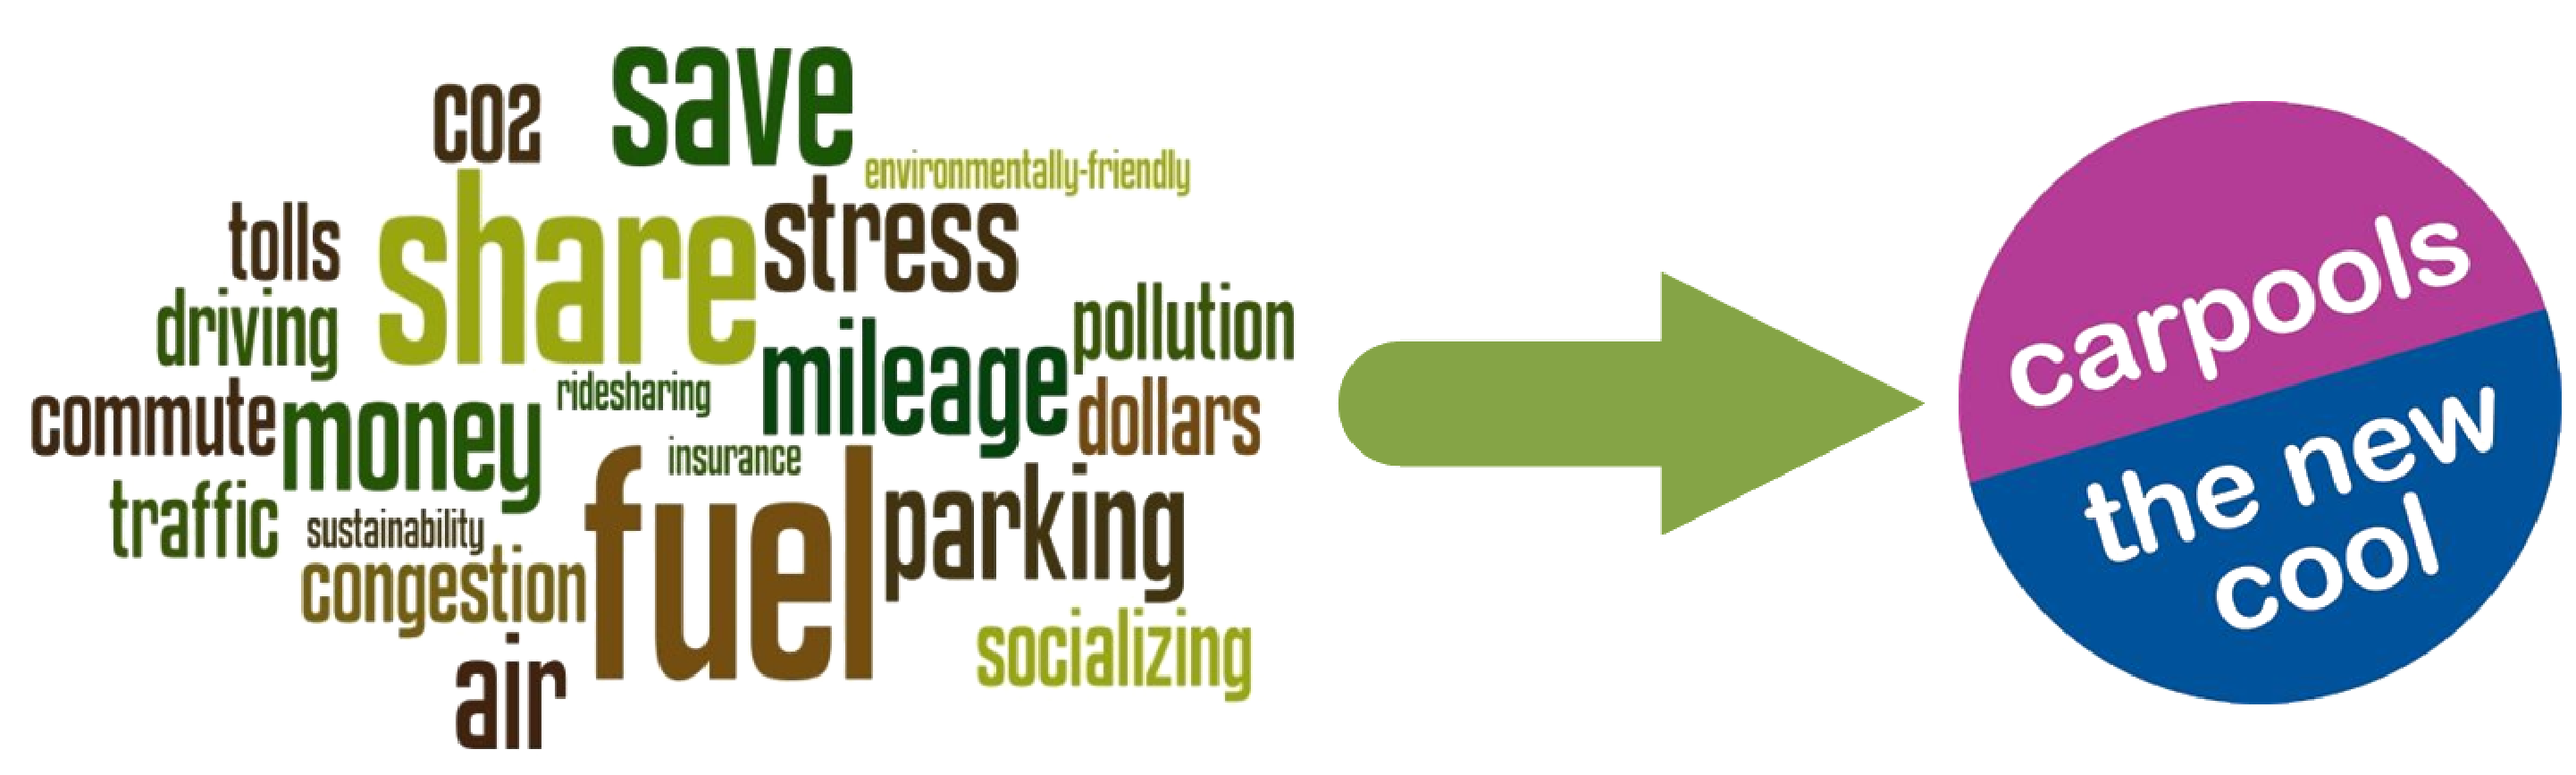
\includegraphics[width = 0.75\columnwidth]{carpool.eps}
\end{figure}
\begin{itemize}
\item<2-> Traditional ride-sharing focused on matching people with similar routes.
\item<3-> Increasing popularity of commercial ride-sharing platforms
\begin{figure}
	\centering
    
\includegraphics[width = 0.55\columnwidth]{ride-sharings.eps}
\end{figure}
\end{itemize}
\end{frame}

\begin{frame}\frametitle{Motivation}
\vspace{-0.28in}
\begin{figure}
	\centering
    
\includegraphics[width = 0.55\columnwidth]{ride-sharings.eps}
\end{figure}
\vspace{-0.23in}
\begin{itemize}
\item Monetary Incentives.
\item<2-> Former studies minimize total traveled distance for drivers:
\begin{itemize}
\item<2-> Riders share fare for carpooling
\only<3-4>{
\begin{figure}
	\centering
    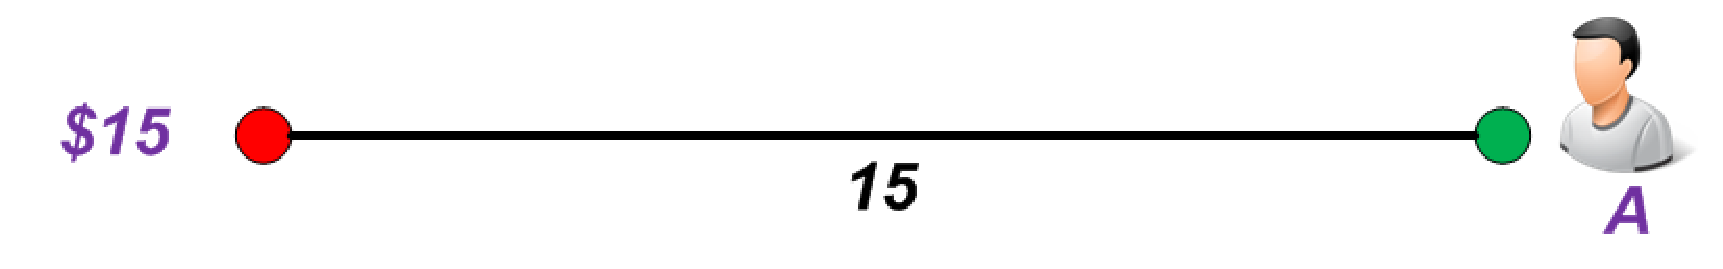
\includegraphics[width = 0.55\columnwidth]{motivation_min1.eps}
\end{figure}
}
\only<4>{
\vspace{-0.1in}
\begin{figure}
	\centering
    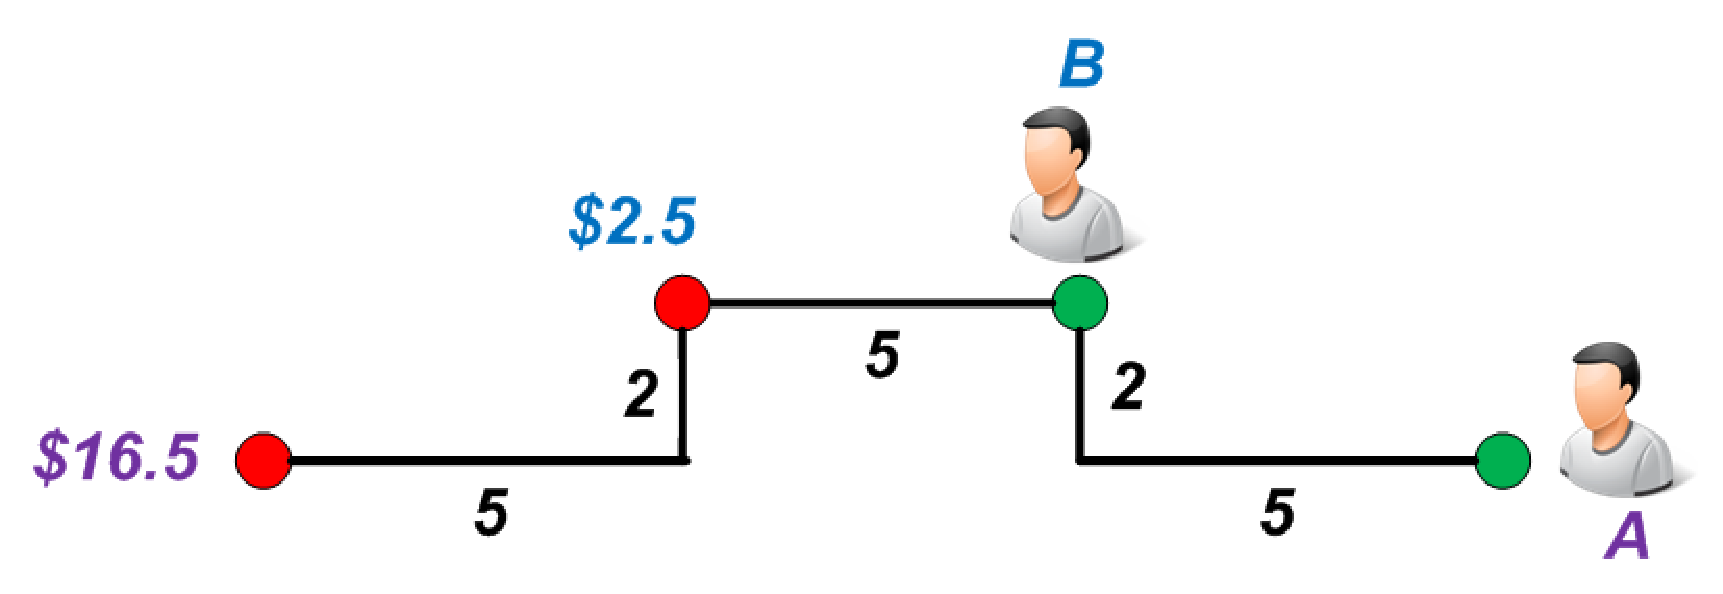
\includegraphics[width = 0.55\columnwidth]{motivation_min2.eps}
\end{figure}
}
\item<5-> Do not account for the service provider's incentive
\end{itemize}
\vspace{-0.1in}
\only<5>{
\begin{figure}
	\centering
   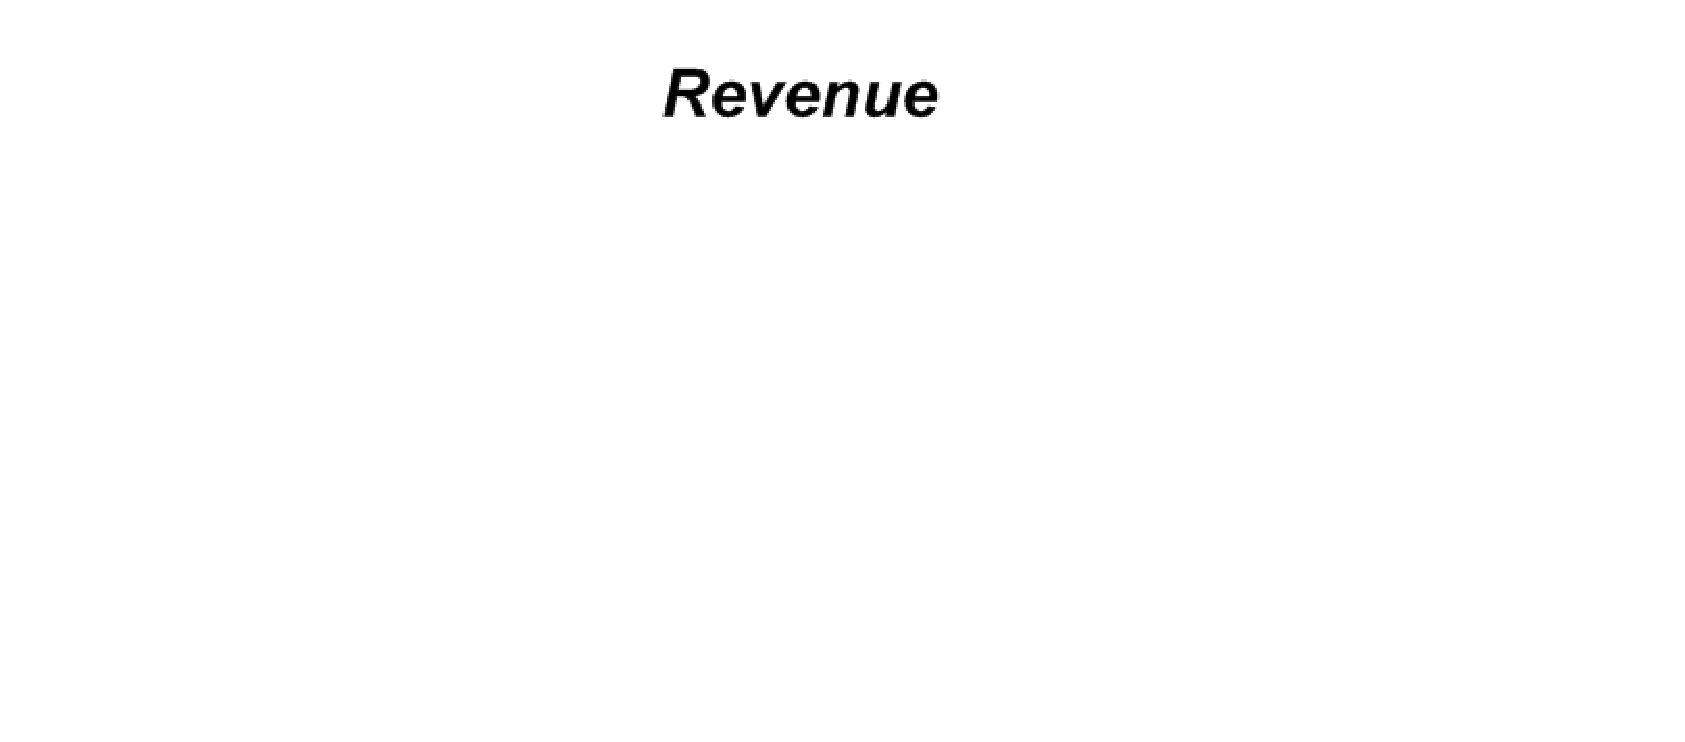
\includegraphics[width = 0.75\columnwidth]{pricing1.eps}
\end{figure}
}
\only<6>{
\begin{figure}
	\centering
    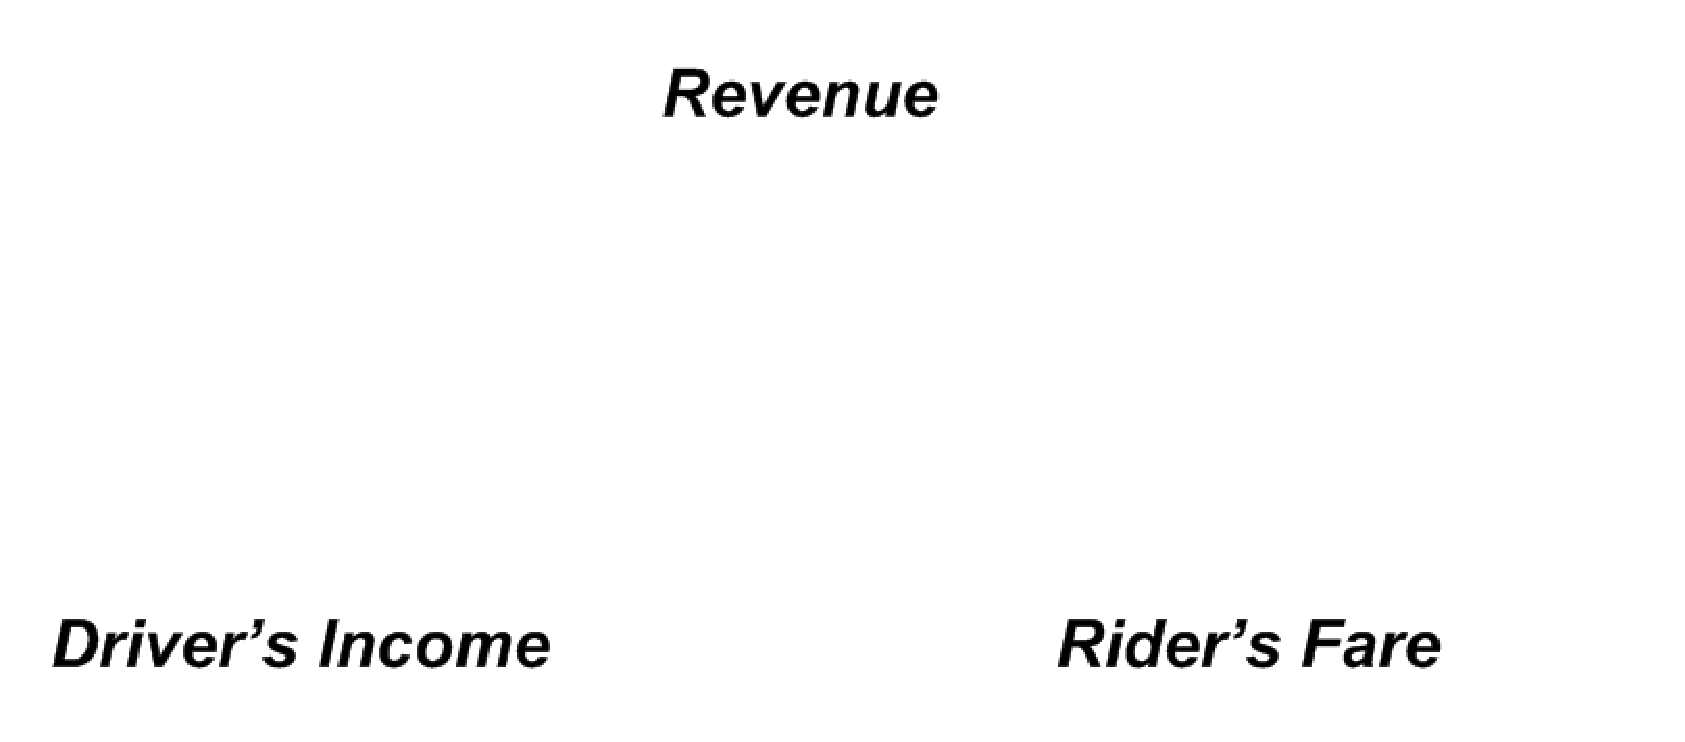
\includegraphics[width = 0.75\columnwidth]{pricing2.eps}
\end{figure}
}
\only<7>{
\begin{figure}
	\centering
    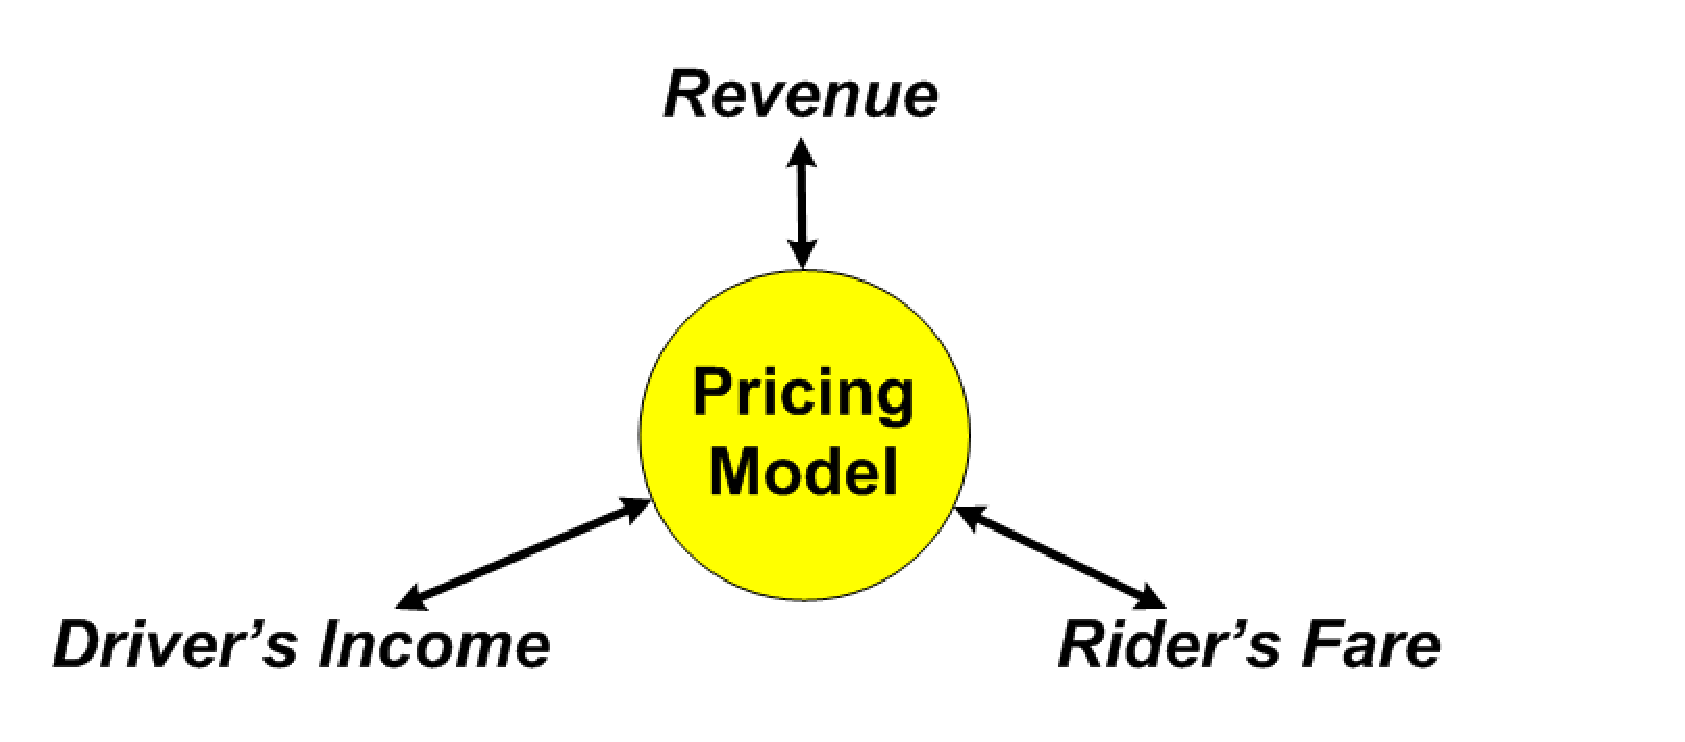
\includegraphics[width = 0.75\columnwidth]{pricing3.eps}
\end{figure}
}
\end{itemize}
\end{frame}

\begin{frame}\frametitle{Motivation}
\vspace{-0.28in}
\begin{figure}
	\centering
    
\includegraphics[width = 0.55\columnwidth]{ride-sharings.eps}
\end{figure}
\vspace{-0.23in}
\begin{itemize}
\item Monetary Incentives.
\item Former studies minimize total traveled distance for drivers:
\begin{itemize}
\item Riders share fare for carpooling
\item Do not account for the service provider's incentive
\end{itemize}
\item Scalability
\only<1>{
\begin{figure}
	\centering
    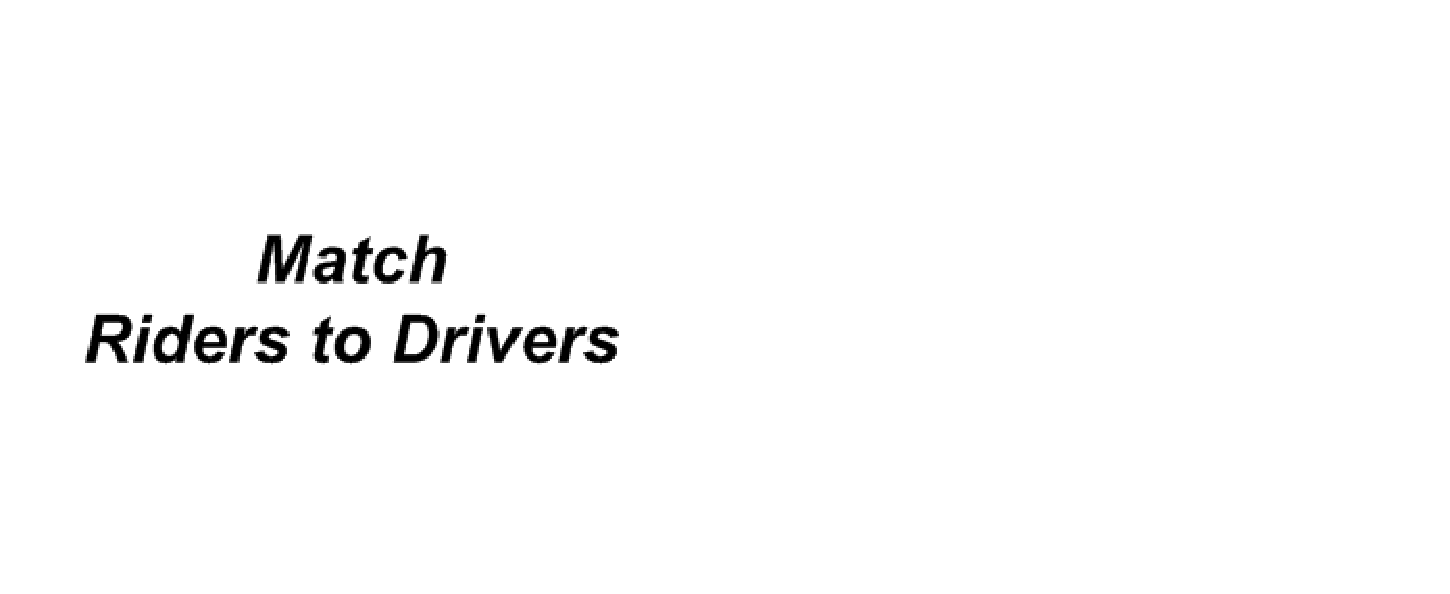
\includegraphics[width = 0.6\columnwidth]{scalability1.eps}
\end{figure}
}
\only<2>{
\begin{figure}
	\centering
    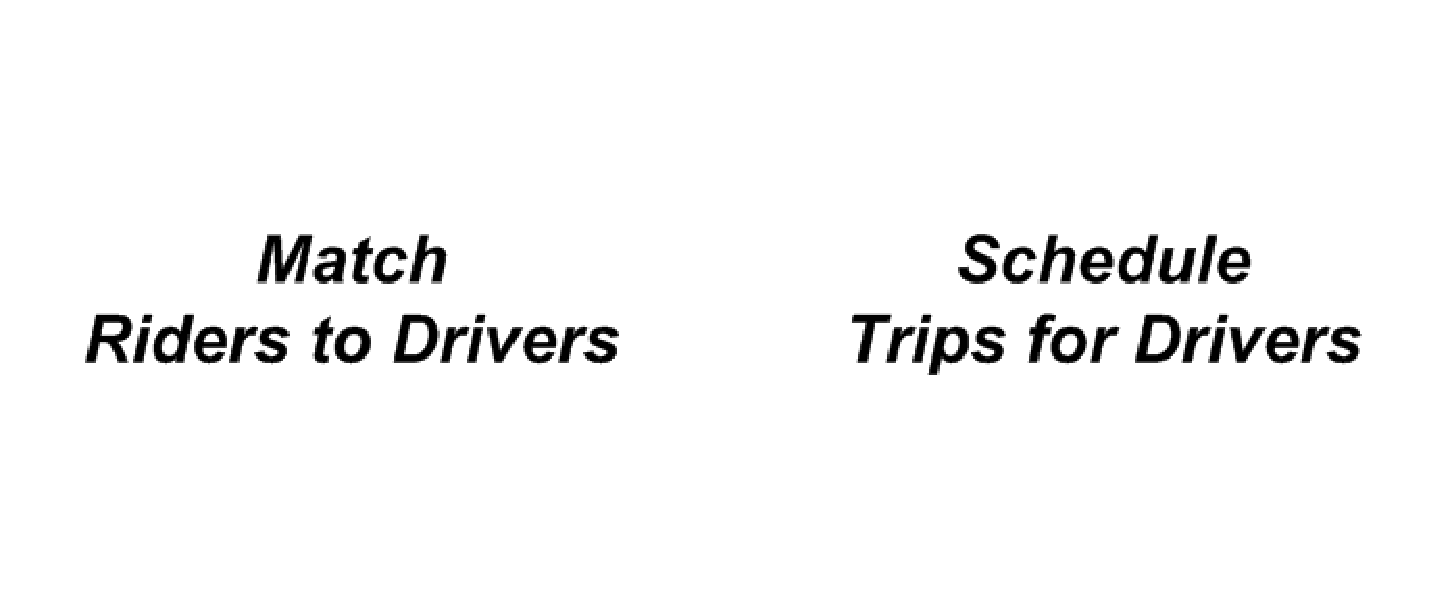
\includegraphics[width = 0.6\columnwidth]{scalability2.eps}
\end{figure}
}
\only<3>{
\begin{figure}
	\centering
    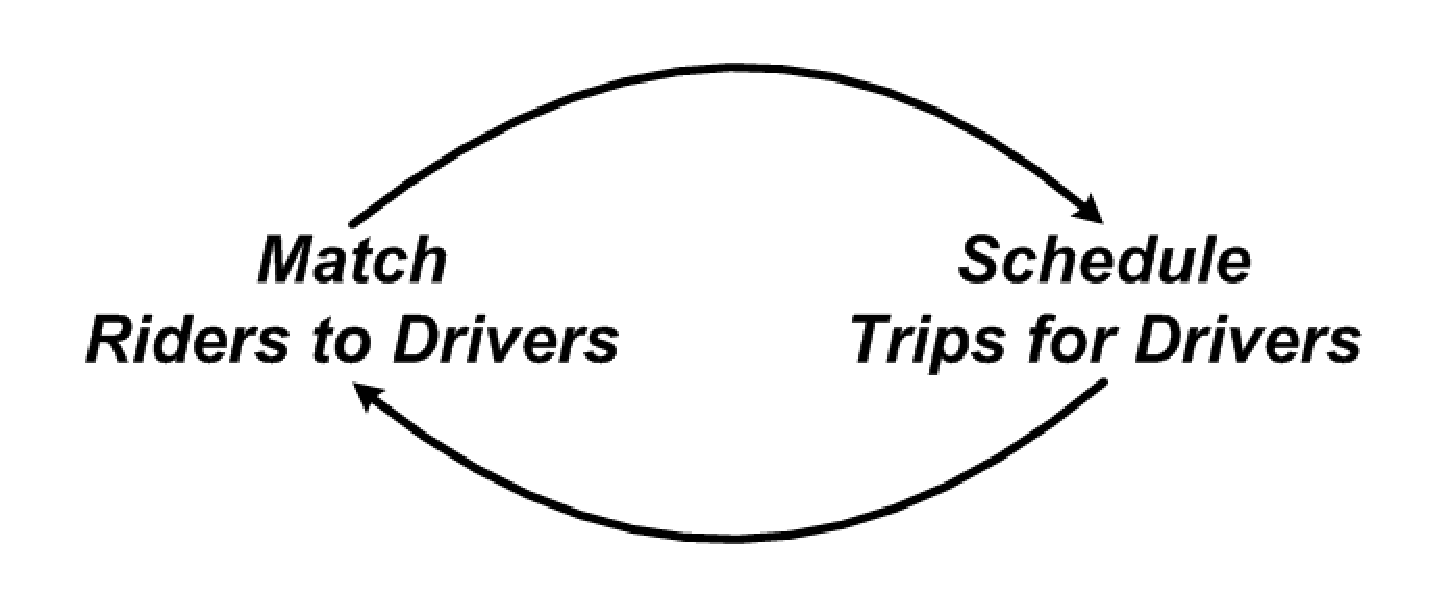
\includegraphics[width = 0.6\columnwidth]{scalability3.eps}
\end{figure}
}
\end{itemize}
\end{frame}

\section{Definitions}
\frame{\frametitle{Outline}\tableofcontents}

\begin{frame}\frametitle{Definitions}
\vspace{-0.2in}
\only<1->{
	\begin{block}{Ride Request}
		A ride request \textit{r} is represented as $\left\langle s, e, w, \epsilon, f \right\rangle$ where:
		\begin{itemize}
			\item \textit{s}: pickup point
			\item \textit{e}: dropoff point
			\item \textit{w}: max wait time
			\item \textit{$\epsilon$}: max detour
			\item \textit{f}: rider's profile
		\end{itemize}			 
	\end{block}
}
\only<2>{
	\begin{alertblock}{Driver}
		A driver \textit{v} is represented as $\left\langle L, n, g \right\rangle$ such that:
		\begin{itemize}
			\item \textit{L}: list of assigned requests
			\item \textit{n}: max simultaneous passengers 
			\item \textit{g}: driver's profile
		\end{itemize}			 
	\end{alertblock}
}
\end{frame}

\begin{frame}\frametitle{Definitions}
\begin{exampleblock}{Schedule}
For a set $L$ with $n$ requests, a schedule $S = \left\langle x_1, x_2, ..., x_2n \right\rangle$ is an ordered set of pickup and dropoff points of the requests in $L$.
\end{exampleblock}

\only<2>{
We call $S$ a \textit{valid} schedule if it satisfies these constraints:
\begin{itemize}
\item for every $r \in L$, $r.s$ precedes $r.e$ in $S$
\item the rider's waiting time and detour
\item the driver's capacity
\end{itemize}
}	

%\tikzoverlay at (3.8cm,2.4cm) {
%        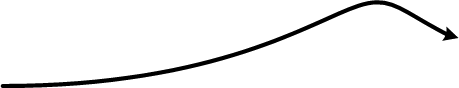
\includegraphics[scale=0.33]{arrow1.png}
%};

\end{frame}

\section{Pricing Model}
\frame{\frametitle{Outline}\tableofcontents[currentsection]}

\begin{frame}\frametitle{Fair Pricing}
For every pricing model:
\begin{itemize}
\item How much should the rider pay?
\item How much should the driver be compensated?
\item What's the revenue of the ride-sharing platform?
\end{itemize}
\vspace{0.5in}
\only<2->{
In a \textit{fair} system:
\begin{itemize}
\item the rider should receive a \textit{discount} proportional the the detour incurred to his trip
\item a driver's compensation should increase proportional to the distance of his trip
\end{itemize}
}
\end{frame}

\begin{frame}\frametitle{Rider's Fare}
for every request \textit{r}:
\begin{itemize}
\item<1-> $d_r$: shortest path between $r.s$ and $r.e$
\item<2-> $F: \mathbb{R}_{+}  \rightarrow \$ $ such that $F(d_r)$ is the default fare of a ride
\end{itemize}
\begin{columns}
\column{0.5\textwidth}
\begin{itemize}
\item<3-> $d'_r$: actual trip of \textit{r}
\item<3-> $\Delta d_r = d'_r - d_r$
\item<4-> $f: \mathbb{R}_{+} \rightarrow \left[ 0, 1 \right] $ specifies the discount for $\Delta d_r \in \mathbb{R}_{+}$
\end{itemize}
\vspace{0.25in}
\only<5->{
\begin{block}{}
\begin{equation*}
fare(r) = F(d_r) f_r(\Delta d_r)
\end{equation*}
\end{block}
}

\column{0.5\textwidth}
\only<5->{
\begin{figure}
	\centering
    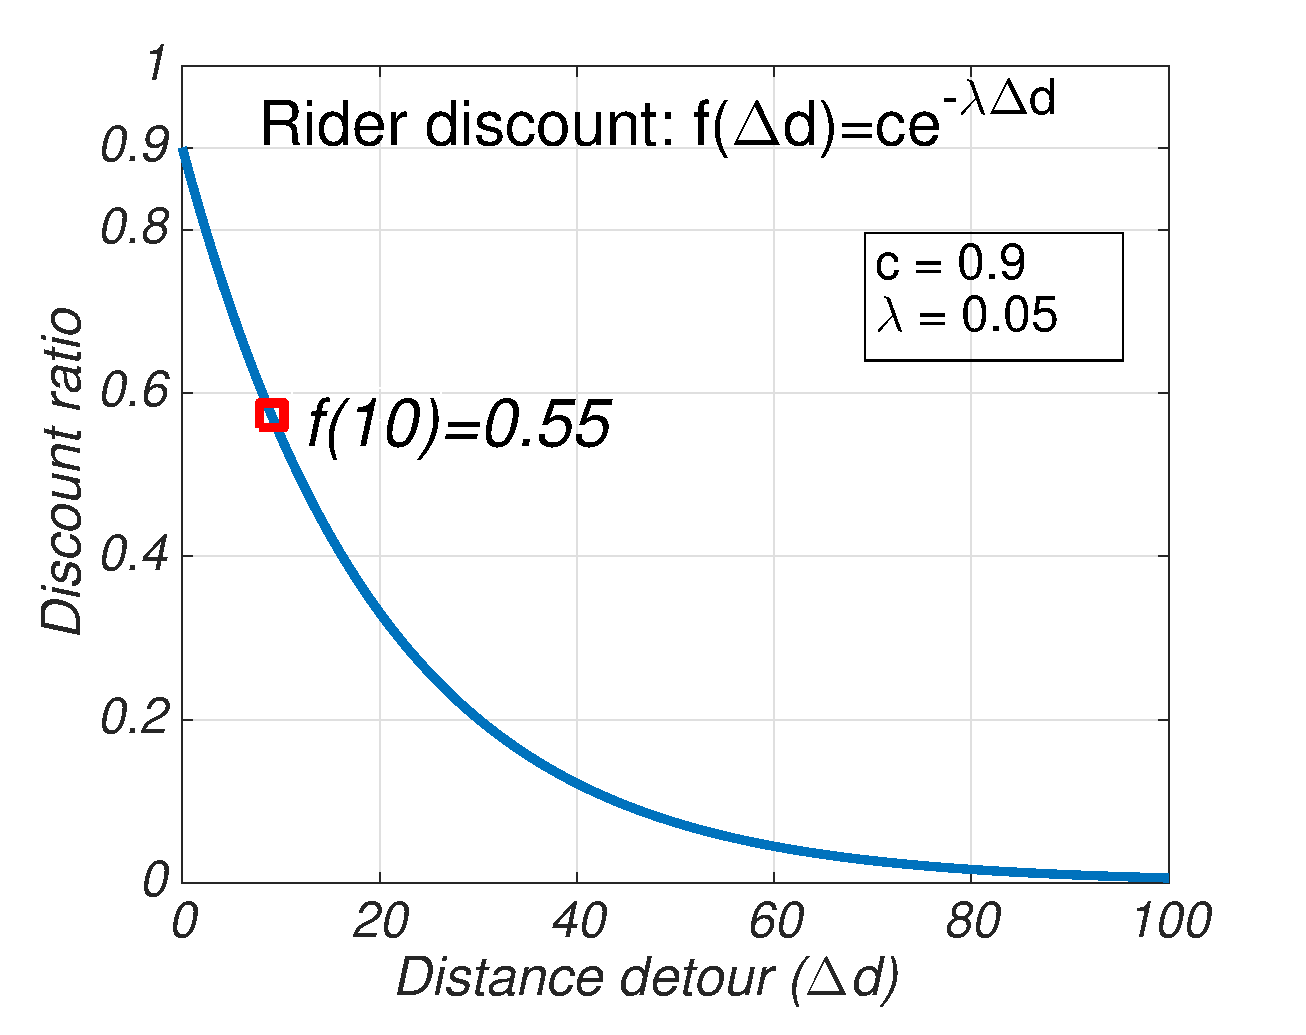
\includegraphics[width = 0.95\columnwidth]{rider.eps}
    \label{fig:quality}
\end{figure}
}
\end{columns}
\end{frame}

\begin{frame}\frametitle{Driver's Income}
\vspace{-0.15in}
for every driver \textit{v}:
\begin{itemize}
\item $g: \mathbb{R}_{+}  \rightarrow \$ $ specifies the monetary cost of \textit{v} driving a distance $d \in \mathbb{R}_{+}$
\begin{itemize}
\item<2-> $g: \mathbb{N} \times \mathbb{R}_{+}  \rightarrow \$$
\end{itemize}
\end{itemize}
\begin{columns}
\column{0.60\textwidth}
\vspace{-0.1in}
\only<4->{
\begin{exampleblock}{}
\begin{equation*}
income_v = \int_{start_s}^{end_s} I\left( S_v(t) \neq \left\langle \right\rangle\right).g(d(t))dt
\end{equation*}
\begin{itemize}
\item $I()$: indicator function
\item $S_v(t)$: driver's schedule at \textit{t}. 
\item $start_s$: first pickup time of $S_v$
\item $end_s$: last dropoff time of $S_v$
\item $d(t)$ traveled distance of \textit{v} at \textit{t}
\end{itemize}
\end{exampleblock}
}
\column{0.40\textwidth}
\only<3->{
\begin{figure}
	\centering
    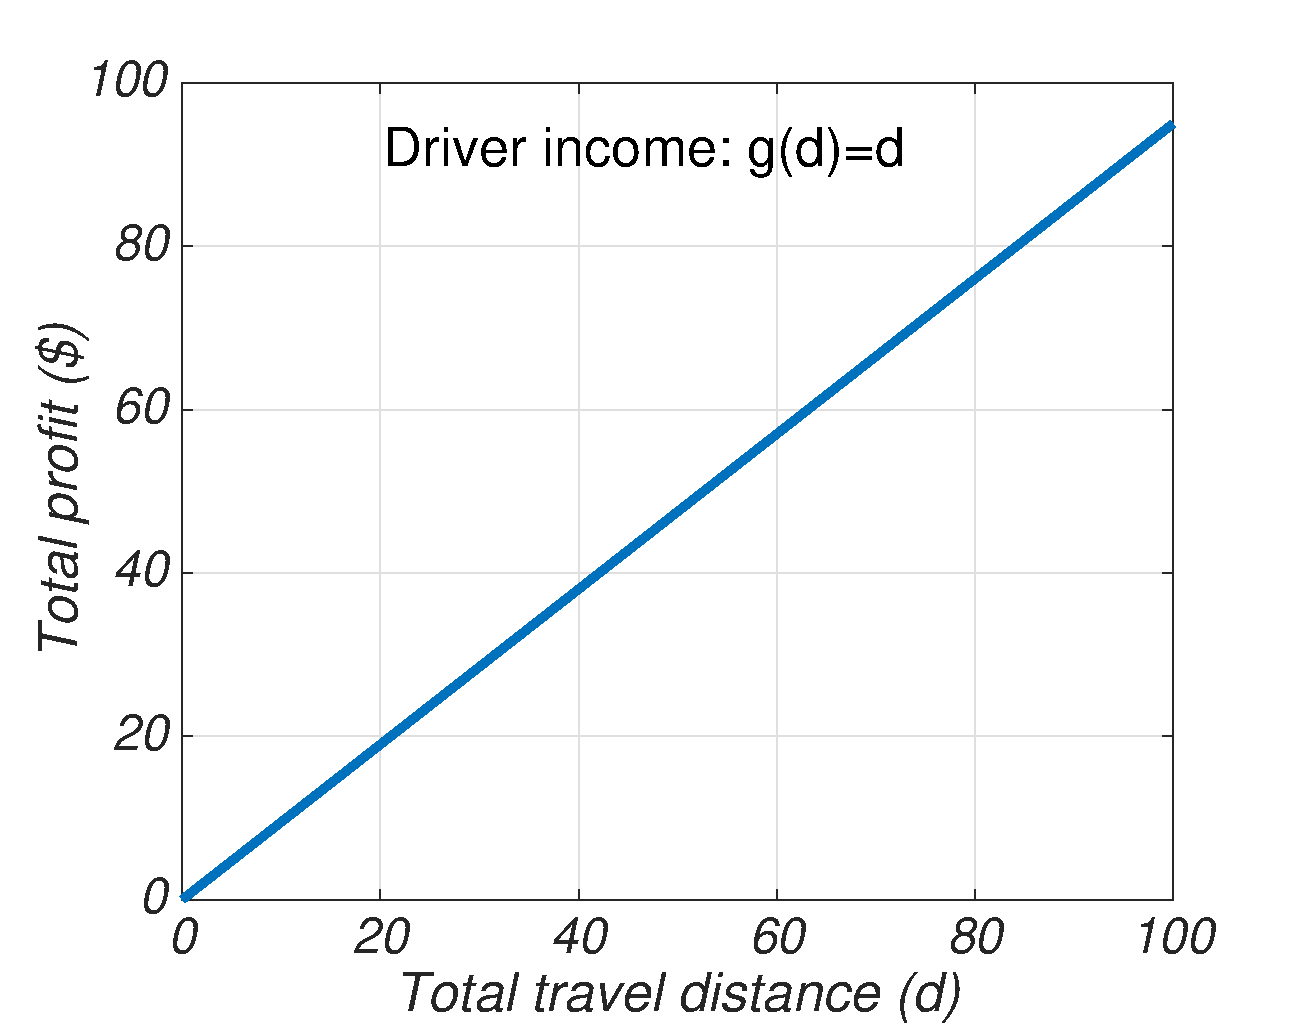
\includegraphics[width = 0.95\columnwidth]{driver.eps}
    \label{fig:quality}
\end{figure}
}
\end{columns}
\end{frame}

\begin{frame}\frametitle{Revenue}
A driver \textit{v}'s profit is:
\begin{equation*}
profit_v = \sum_{r_i \in S_v}fare(r_i) - income_v
\end{equation*}
\vspace{0.5in}
\only<2->{
therefore,
\begin{equation*}
revenue = \sum_{v \in V}profit_v
\end{equation*}
}
\end{frame}

\section{APART Framework}
\frame{\frametitle{Outline}\tableofcontents[currentsection]}

\begin{frame}\frametitle{Overview}
\only<1>{
\vspace{-0.15in}
\begin{figure}
	\centering
    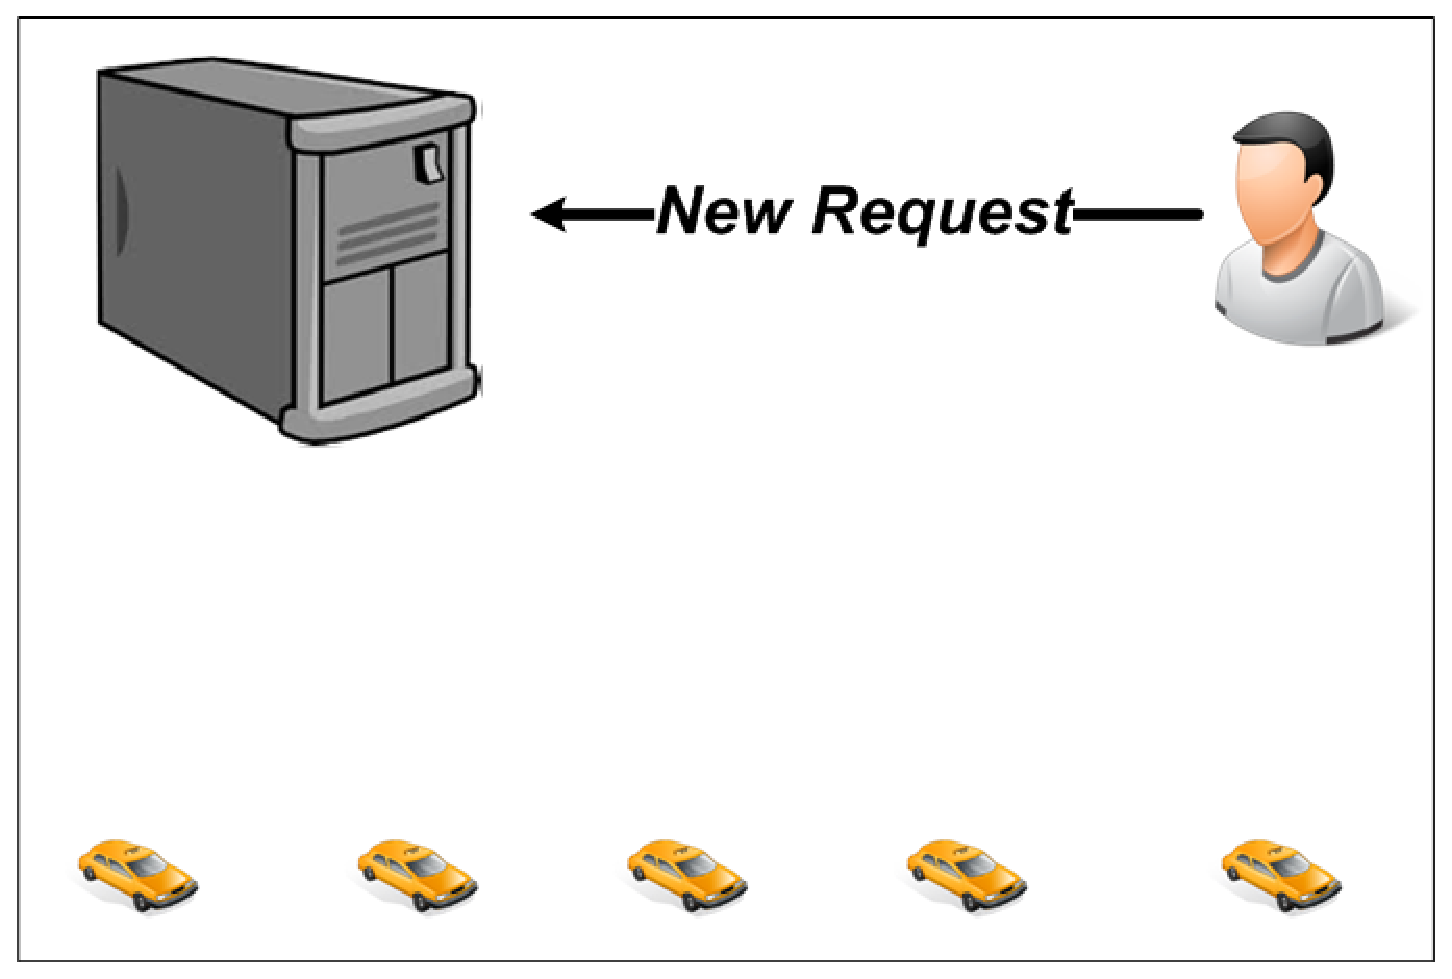
\includegraphics[width = 0.95\columnwidth]{overview1.eps}
\end{figure}
}
\only<2>{
\vspace{-0.15in}
\begin{figure}
	\centering
    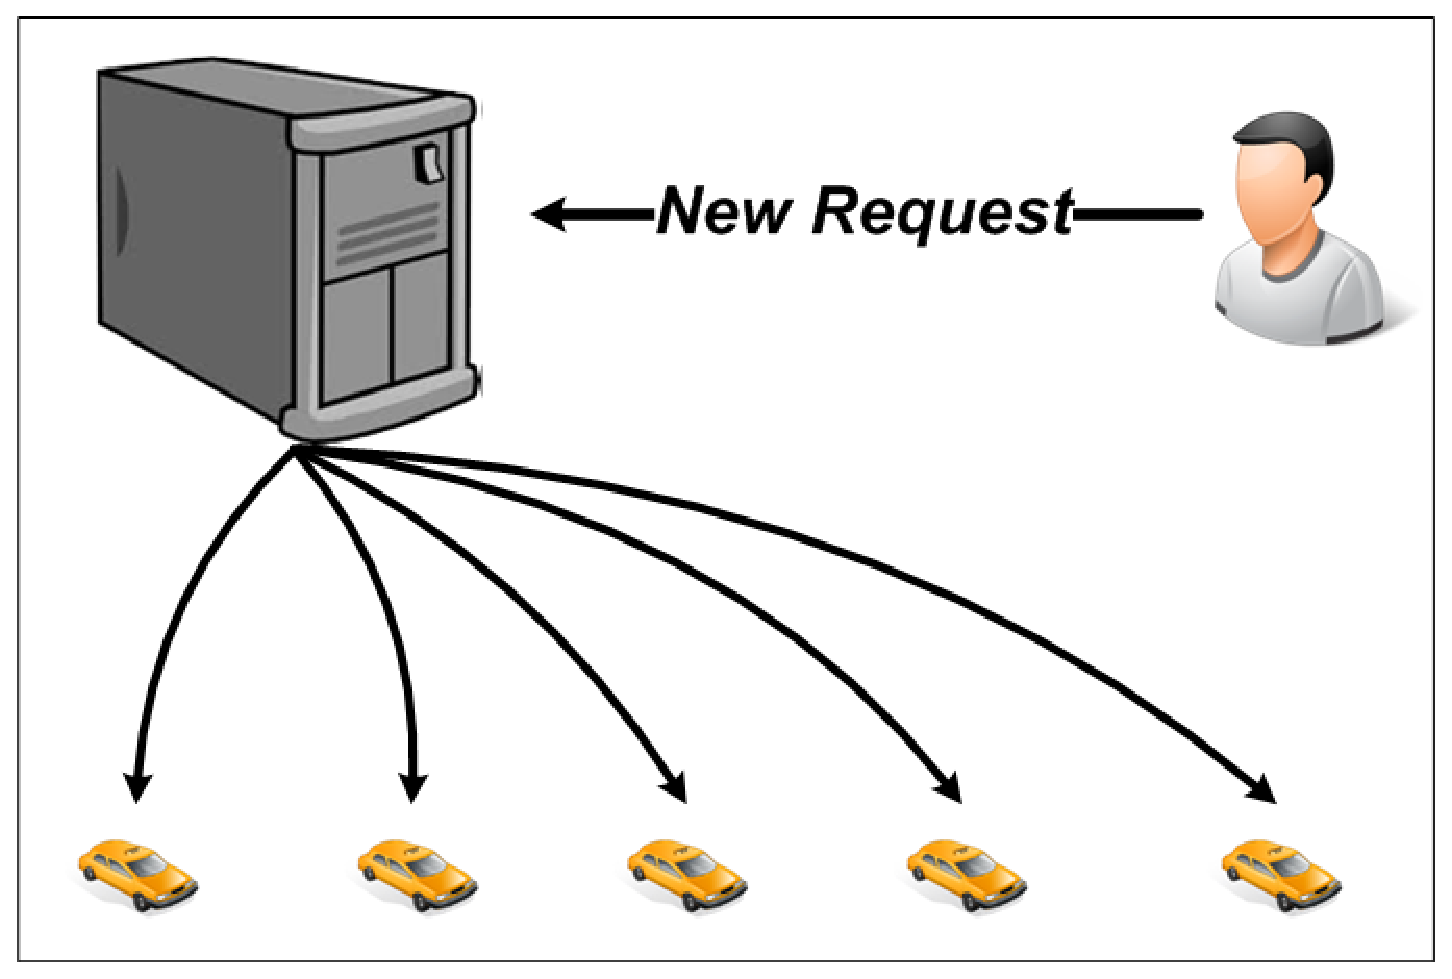
\includegraphics[width = 0.95\columnwidth]{overview2.eps}
\end{figure}
}
\only<3>{
\vspace{-0.15in}
\begin{figure}
	\centering
    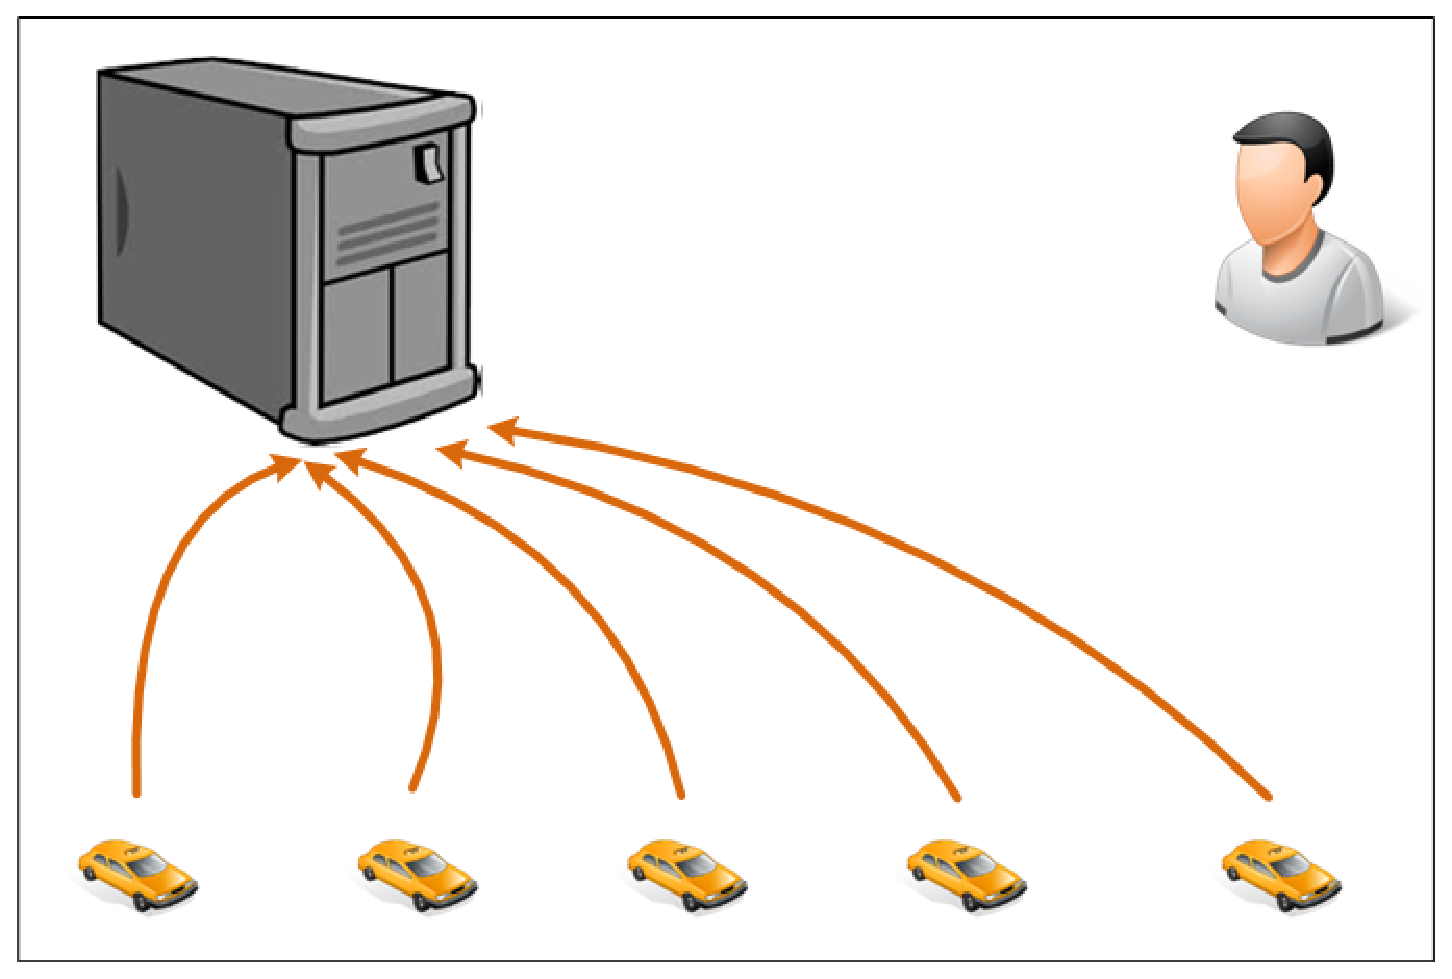
\includegraphics[width = 0.95\columnwidth]{overview3.eps}
\end{figure}
}
\only<4>{
\vspace{-0.15in}
\begin{figure}
	\centering
    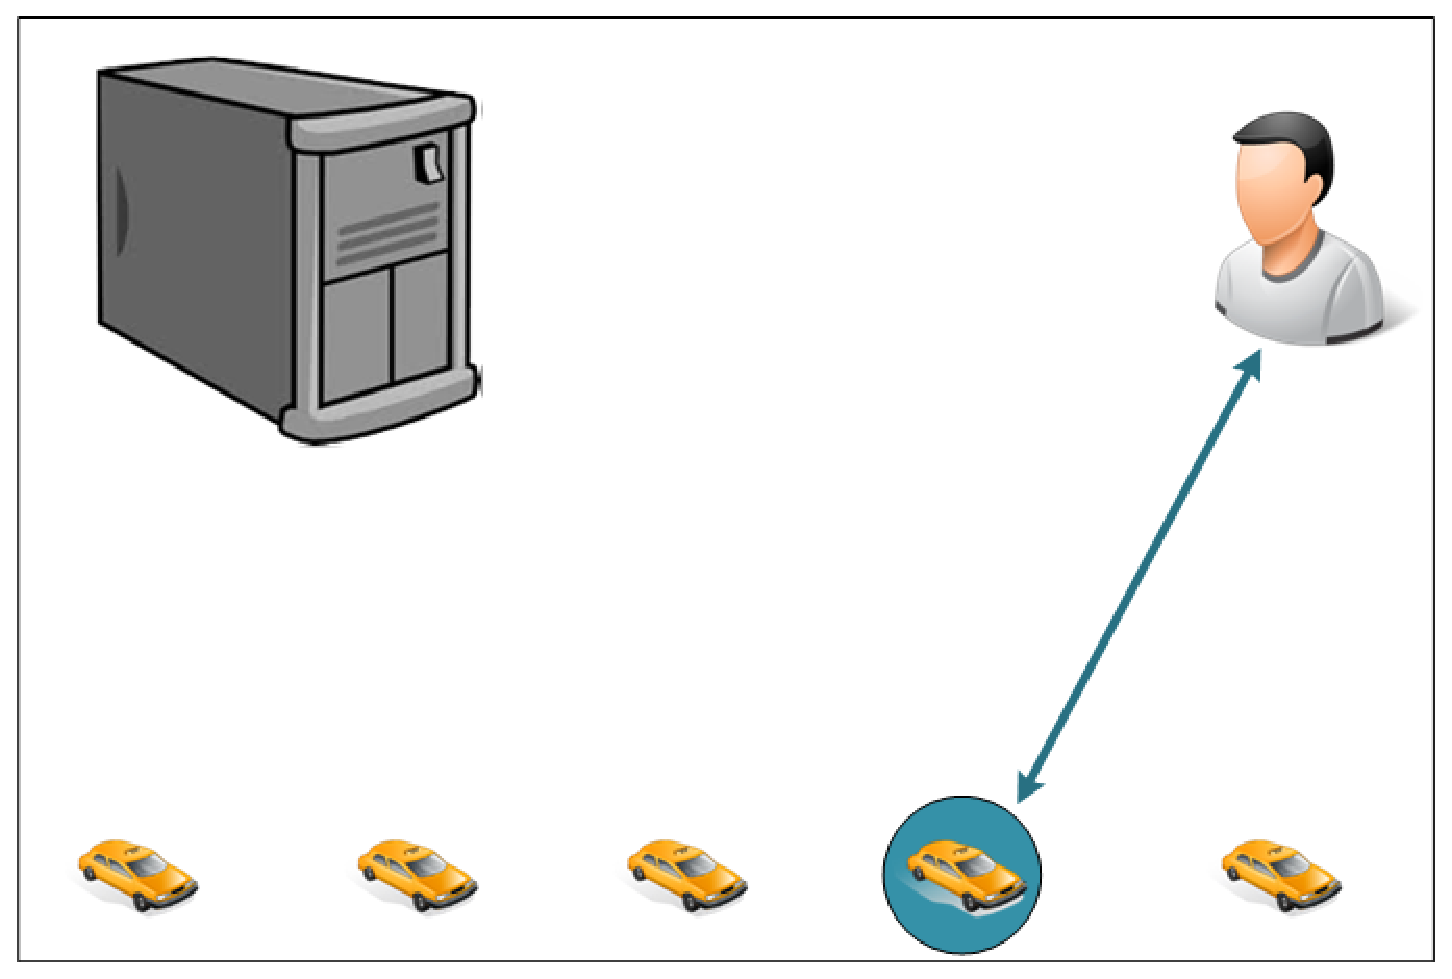
\includegraphics[width = 0.95\columnwidth]{overview4.eps}
\end{figure}
}
\end{frame}

\begin{frame}\frametitle{Dispatching Tasks}
\only<1>{
\vspace{-0.15in}
\begin{figure}
	\centering
    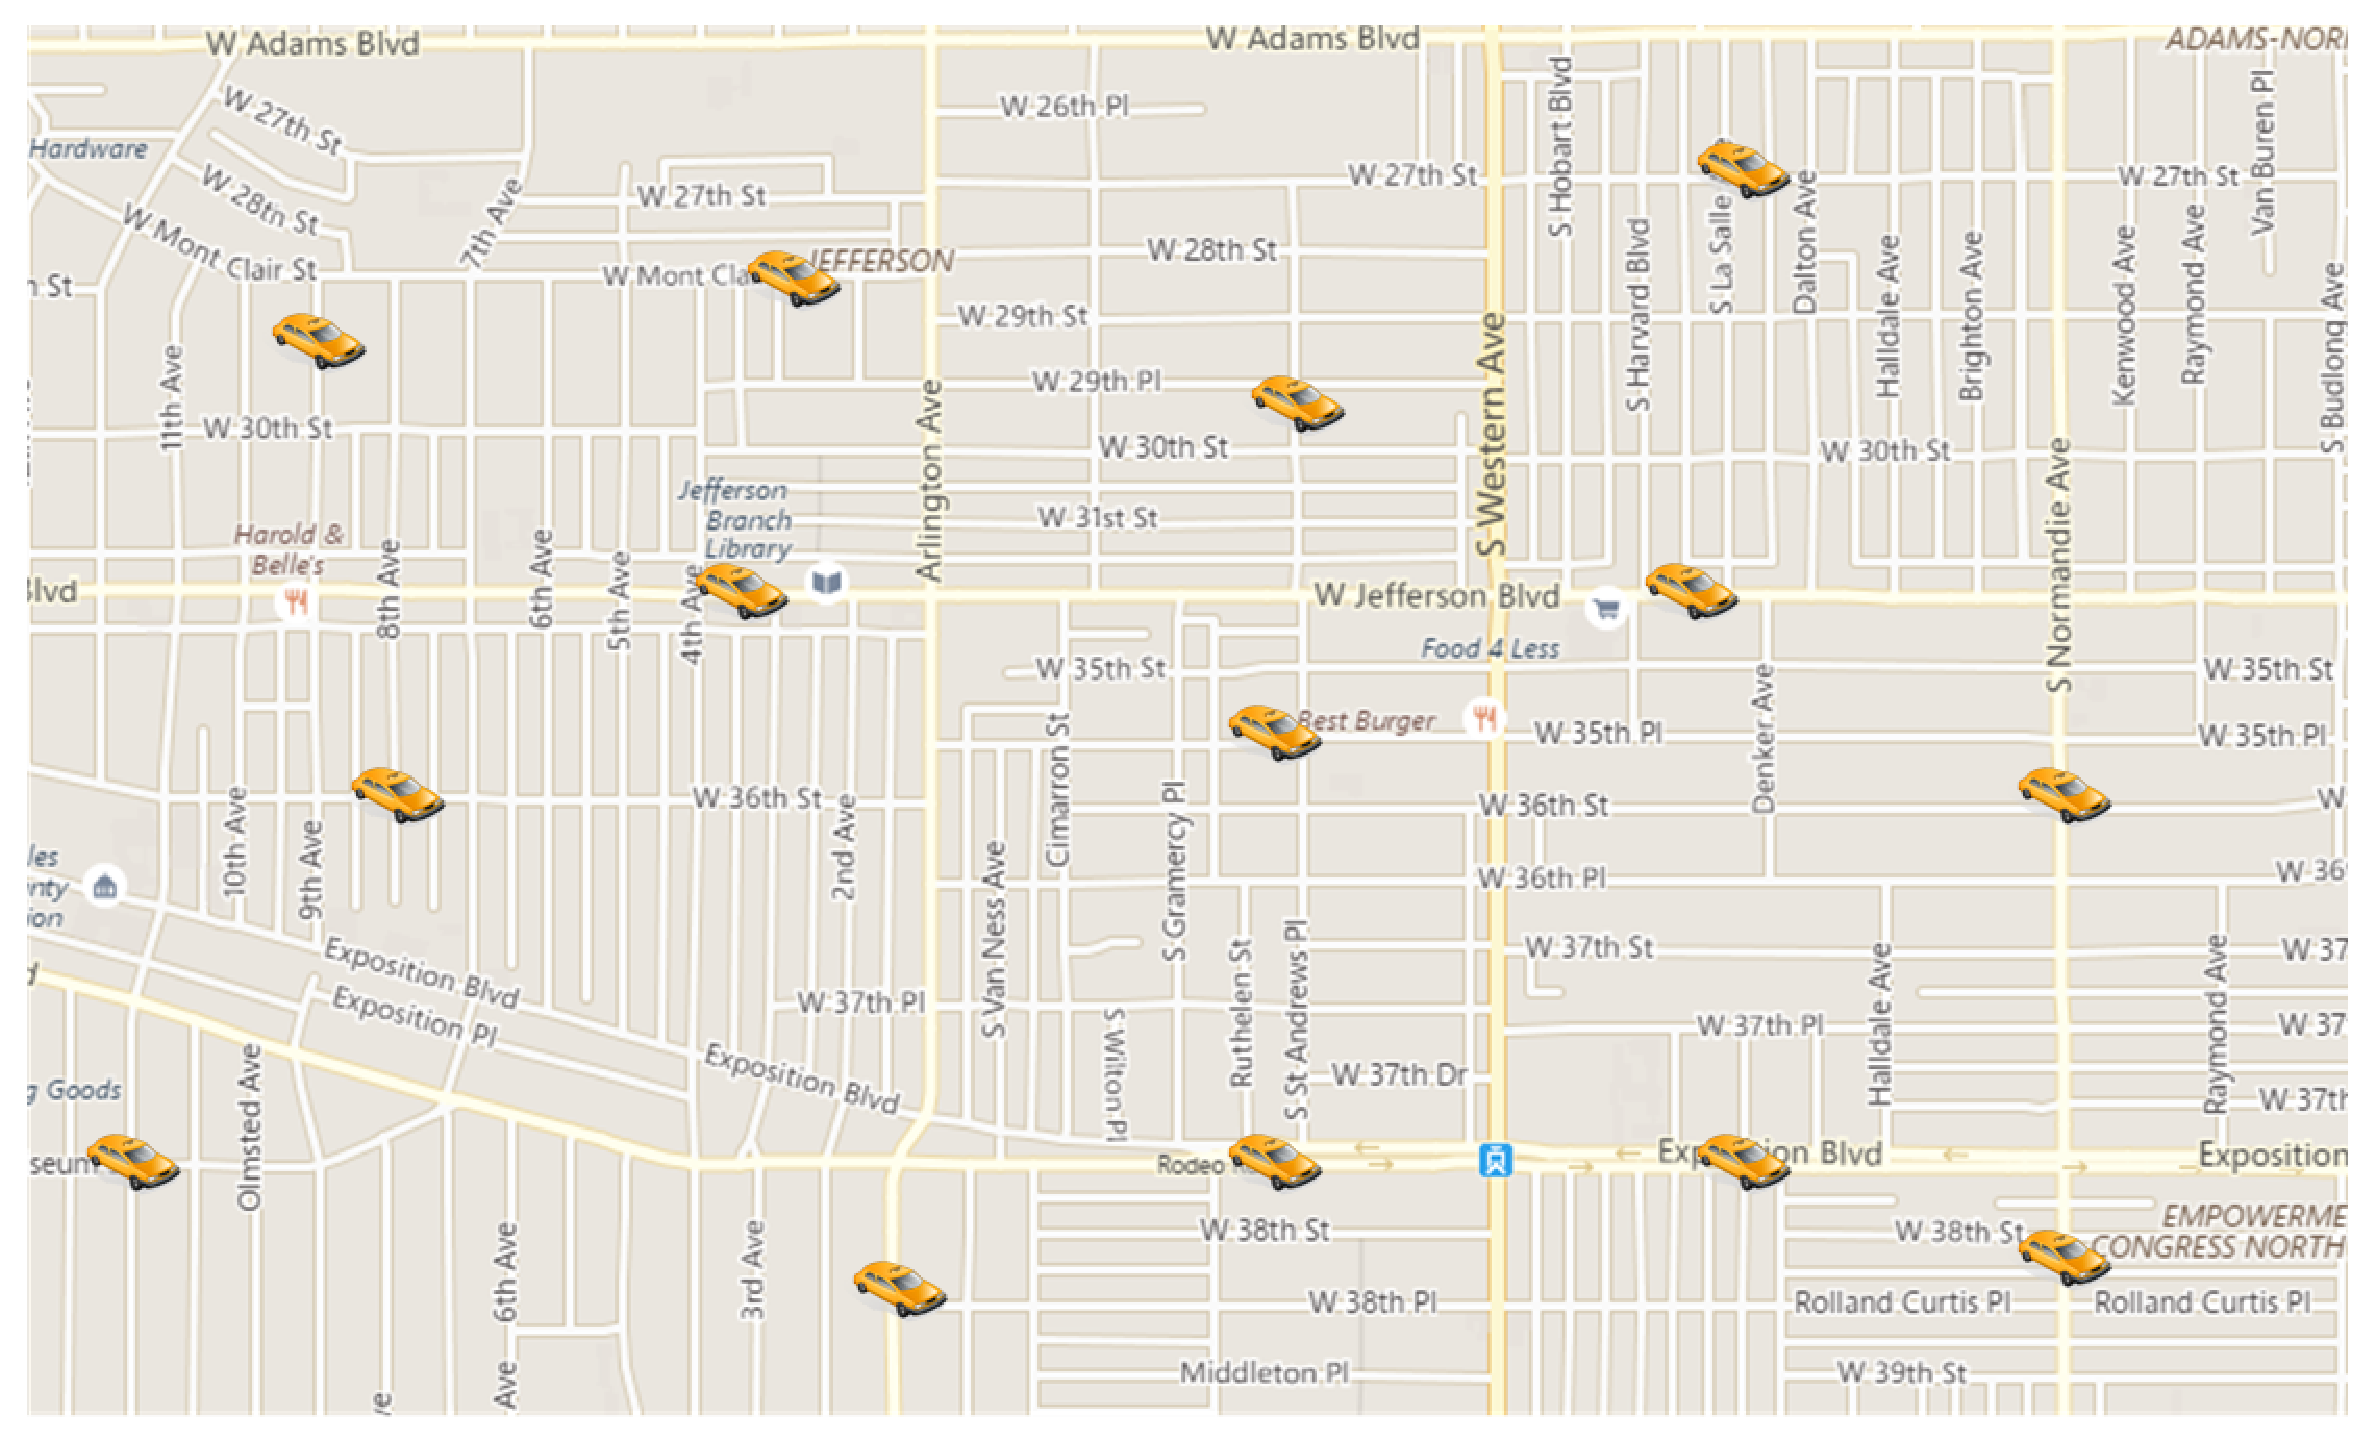
\includegraphics[width = 0.95\columnwidth]{dispatch1.eps}
\end{figure}
}
\only<2>{
\vspace{-0.15in}
\begin{figure}
	\centering
    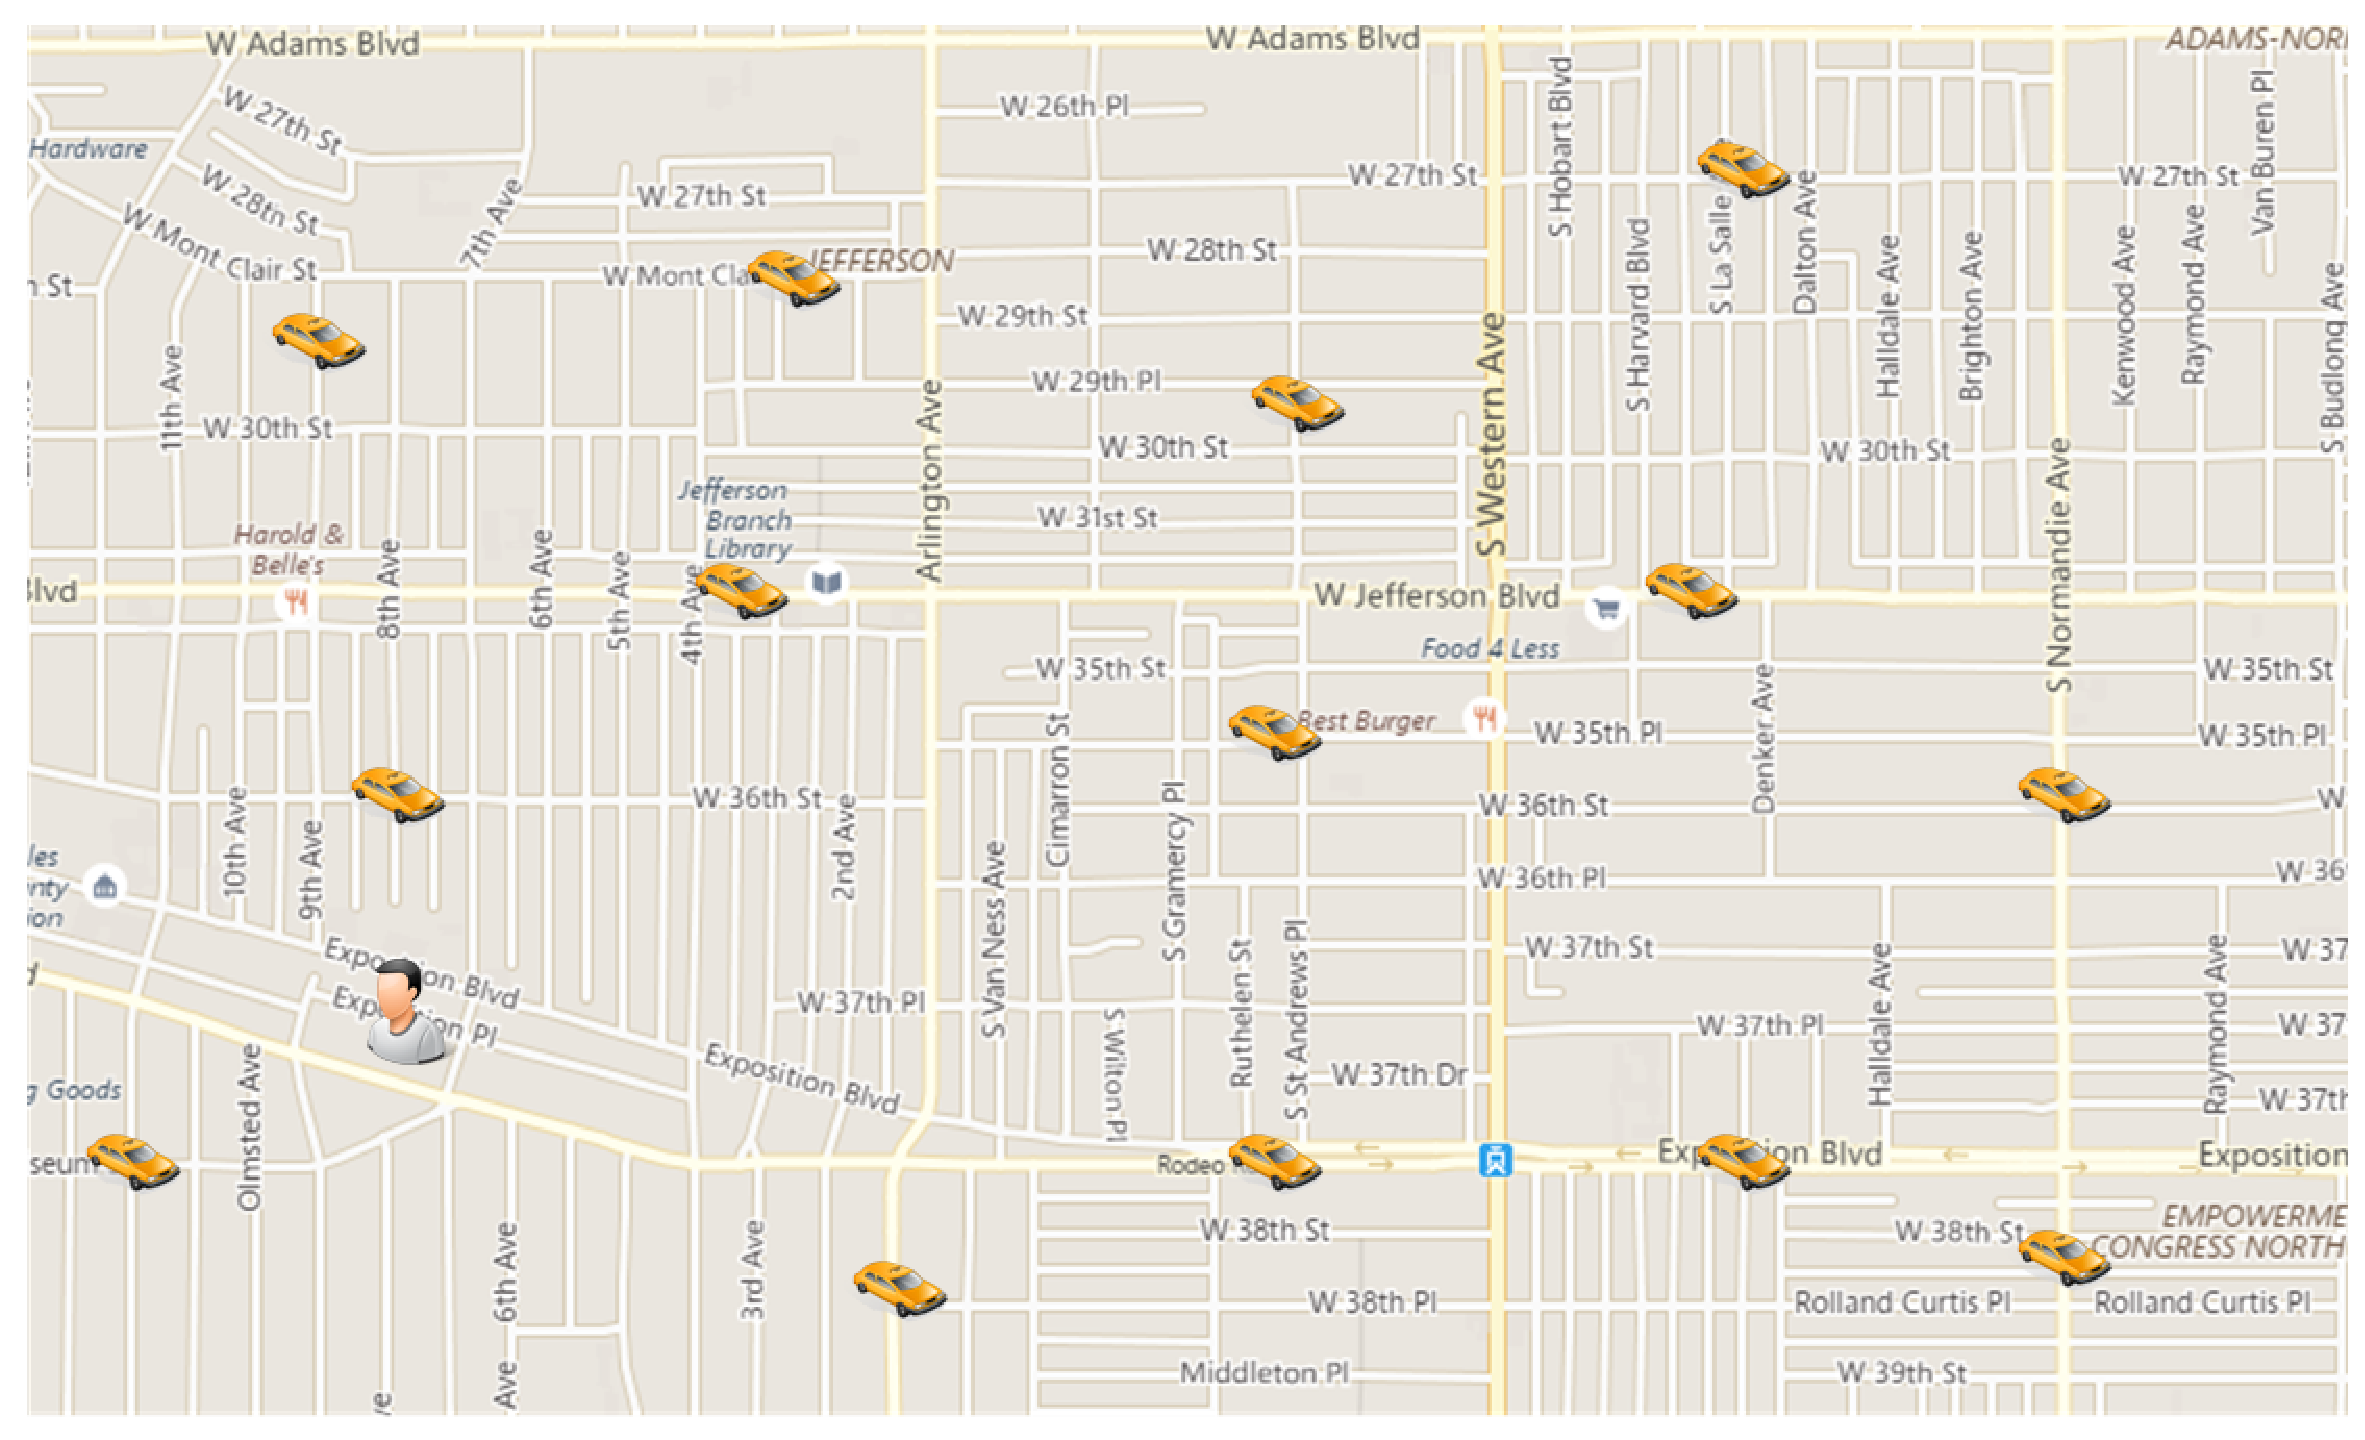
\includegraphics[width = 0.95\columnwidth]{dispatch2.eps}
\end{figure}
}
%\only<3>{
%\vspace{-0.15in}
%\begin{figure}
%	\centering
%   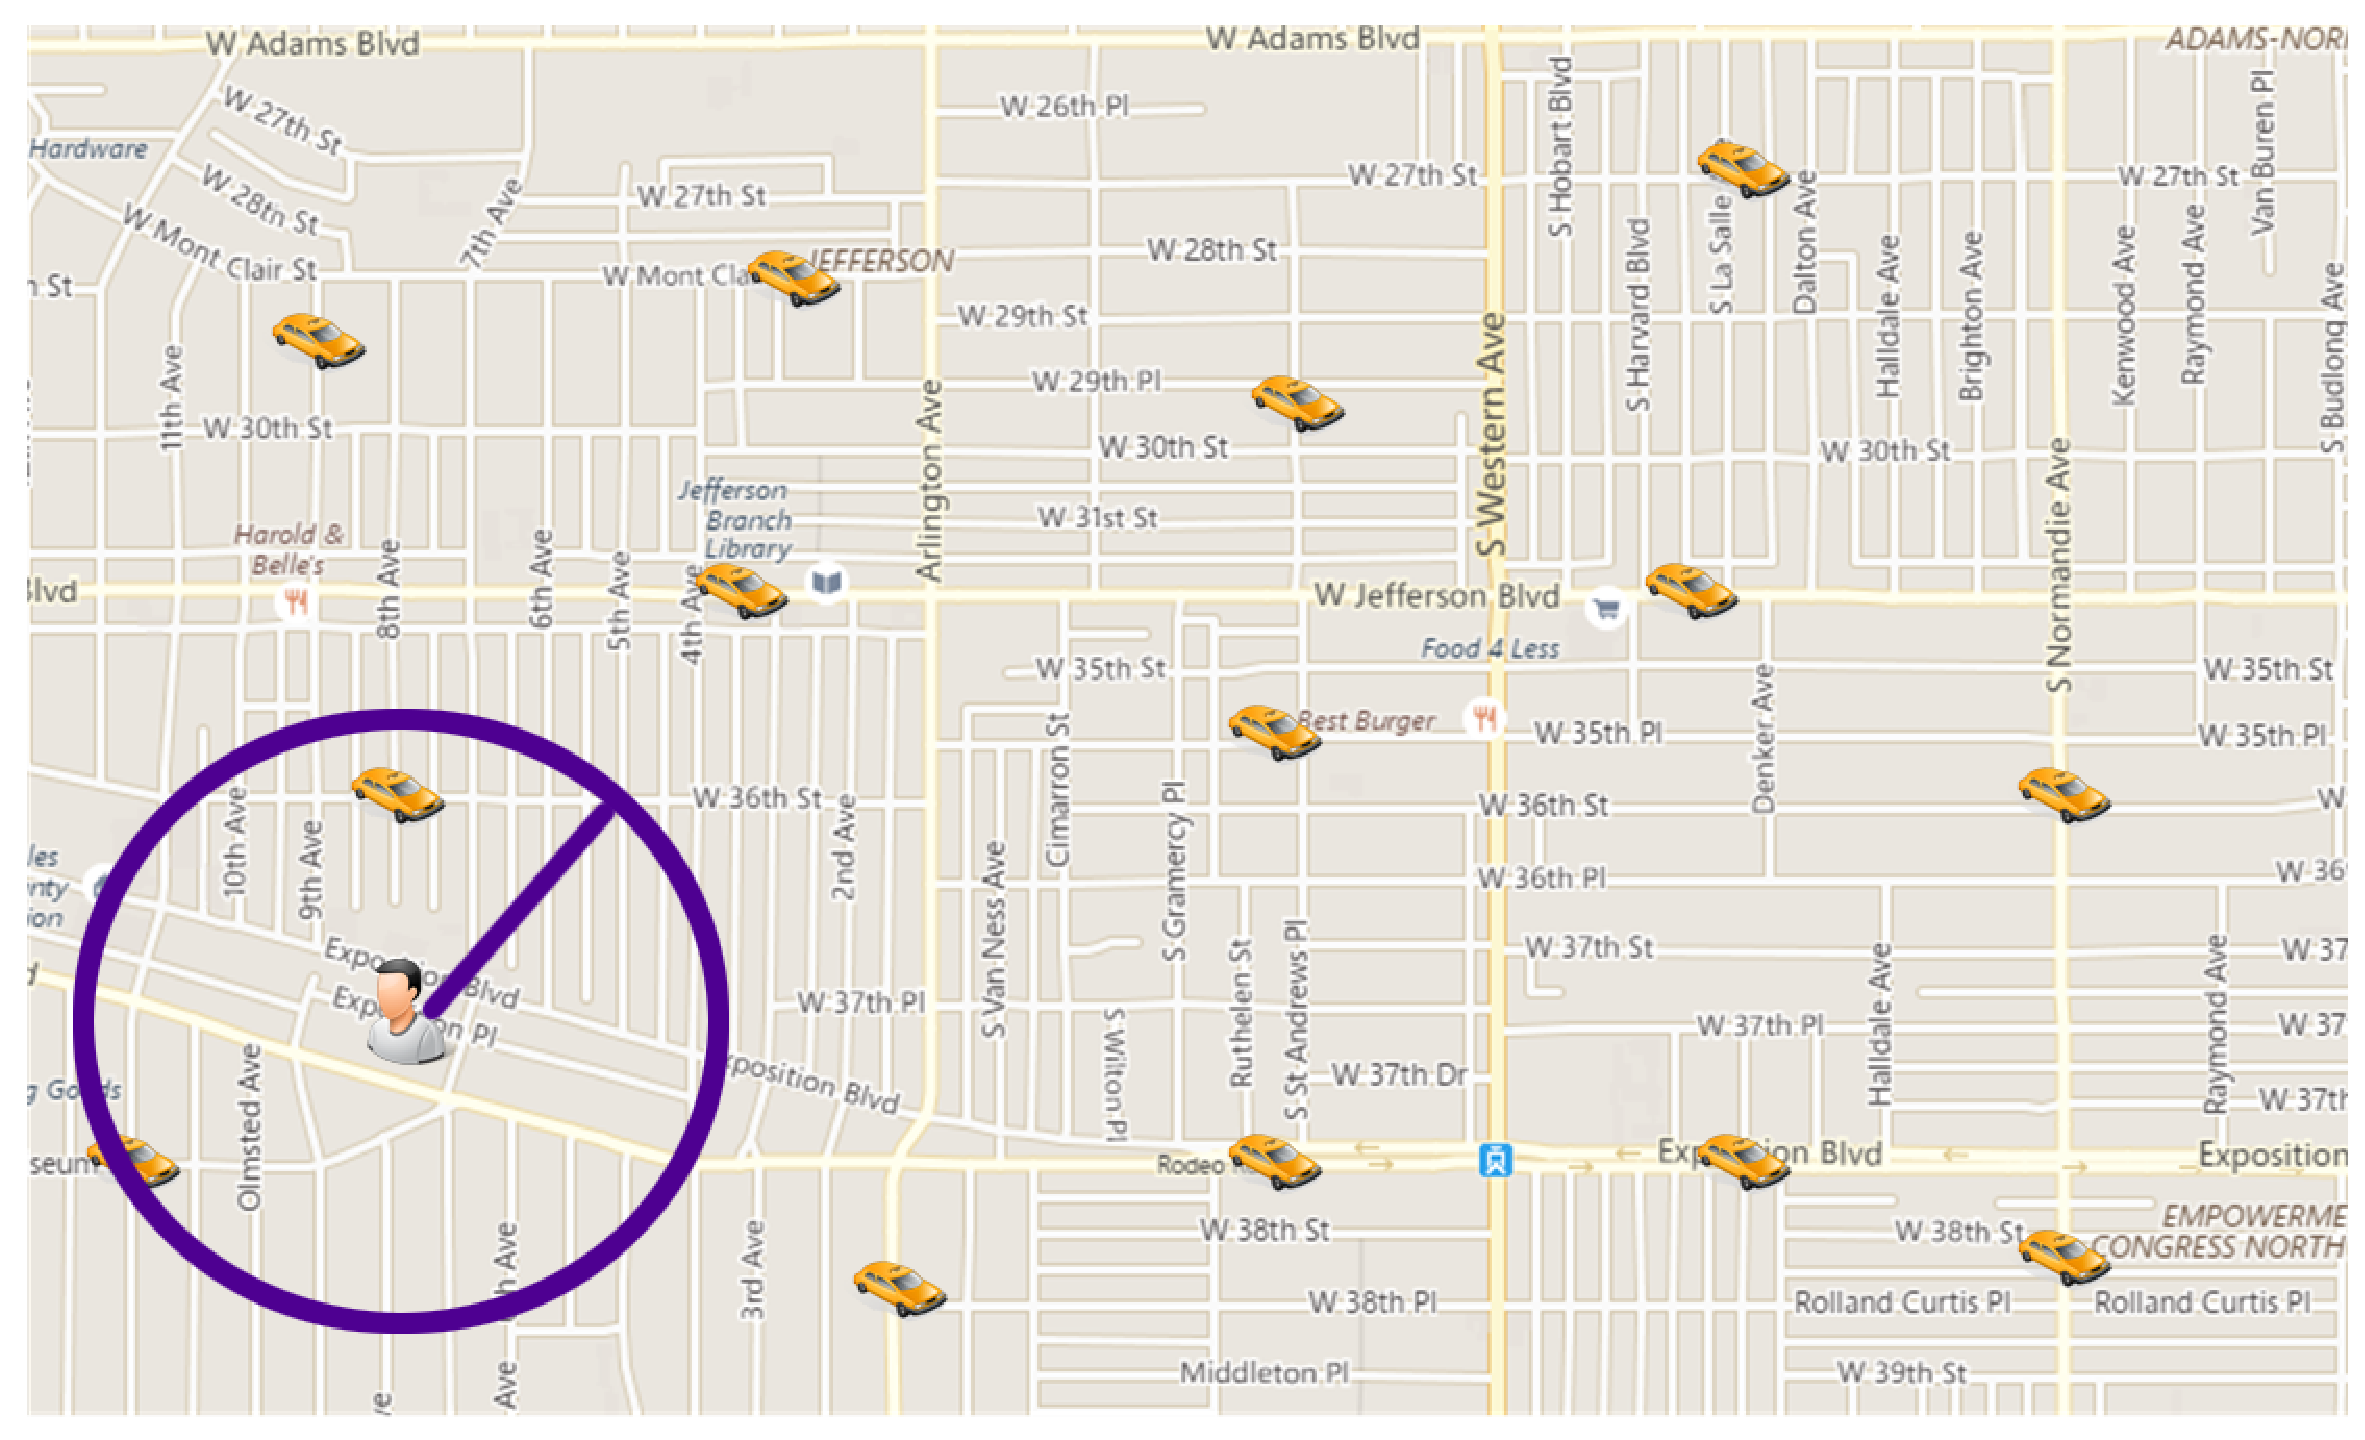
\includegraphics[width = 0.95\columnwidth]{dispatch3.eps}
%\end{figure}
%}
\only<3>{
\vspace{-0.15in}
\begin{figure}
	\centering
    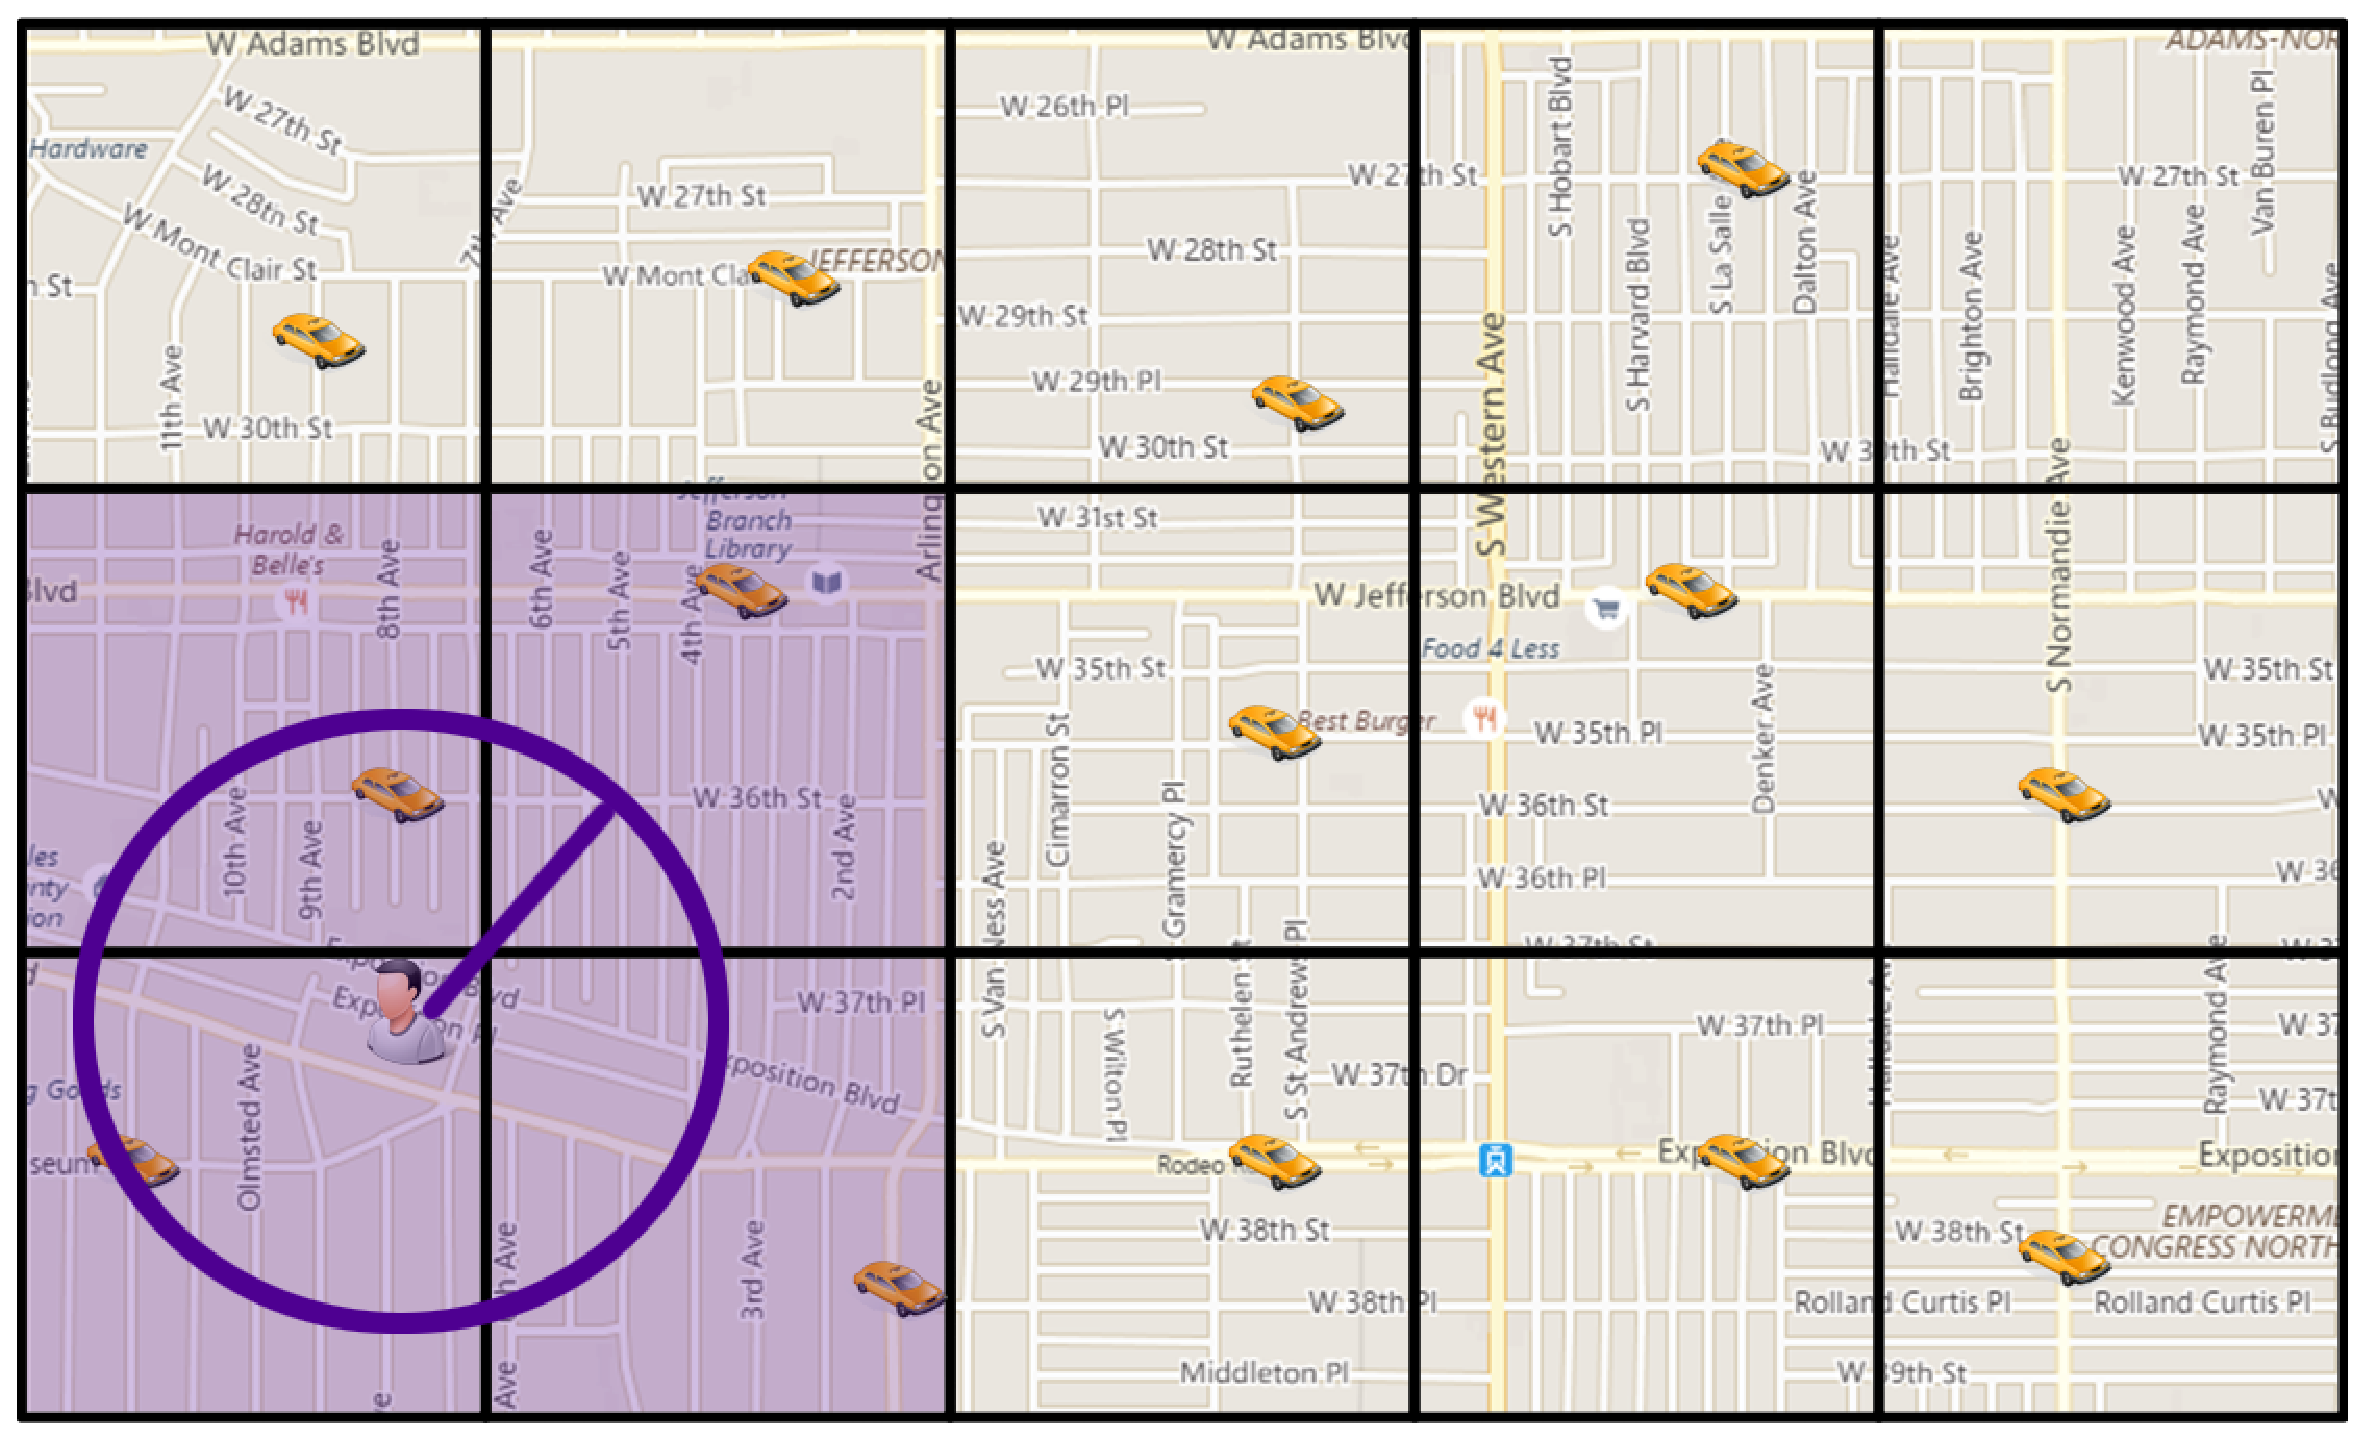
\includegraphics[width = 0.95\columnwidth]{dispatch4.eps}
\end{figure}
}
\only<4>{
\vspace{-0.15in}
\begin{figure}
	\centering
    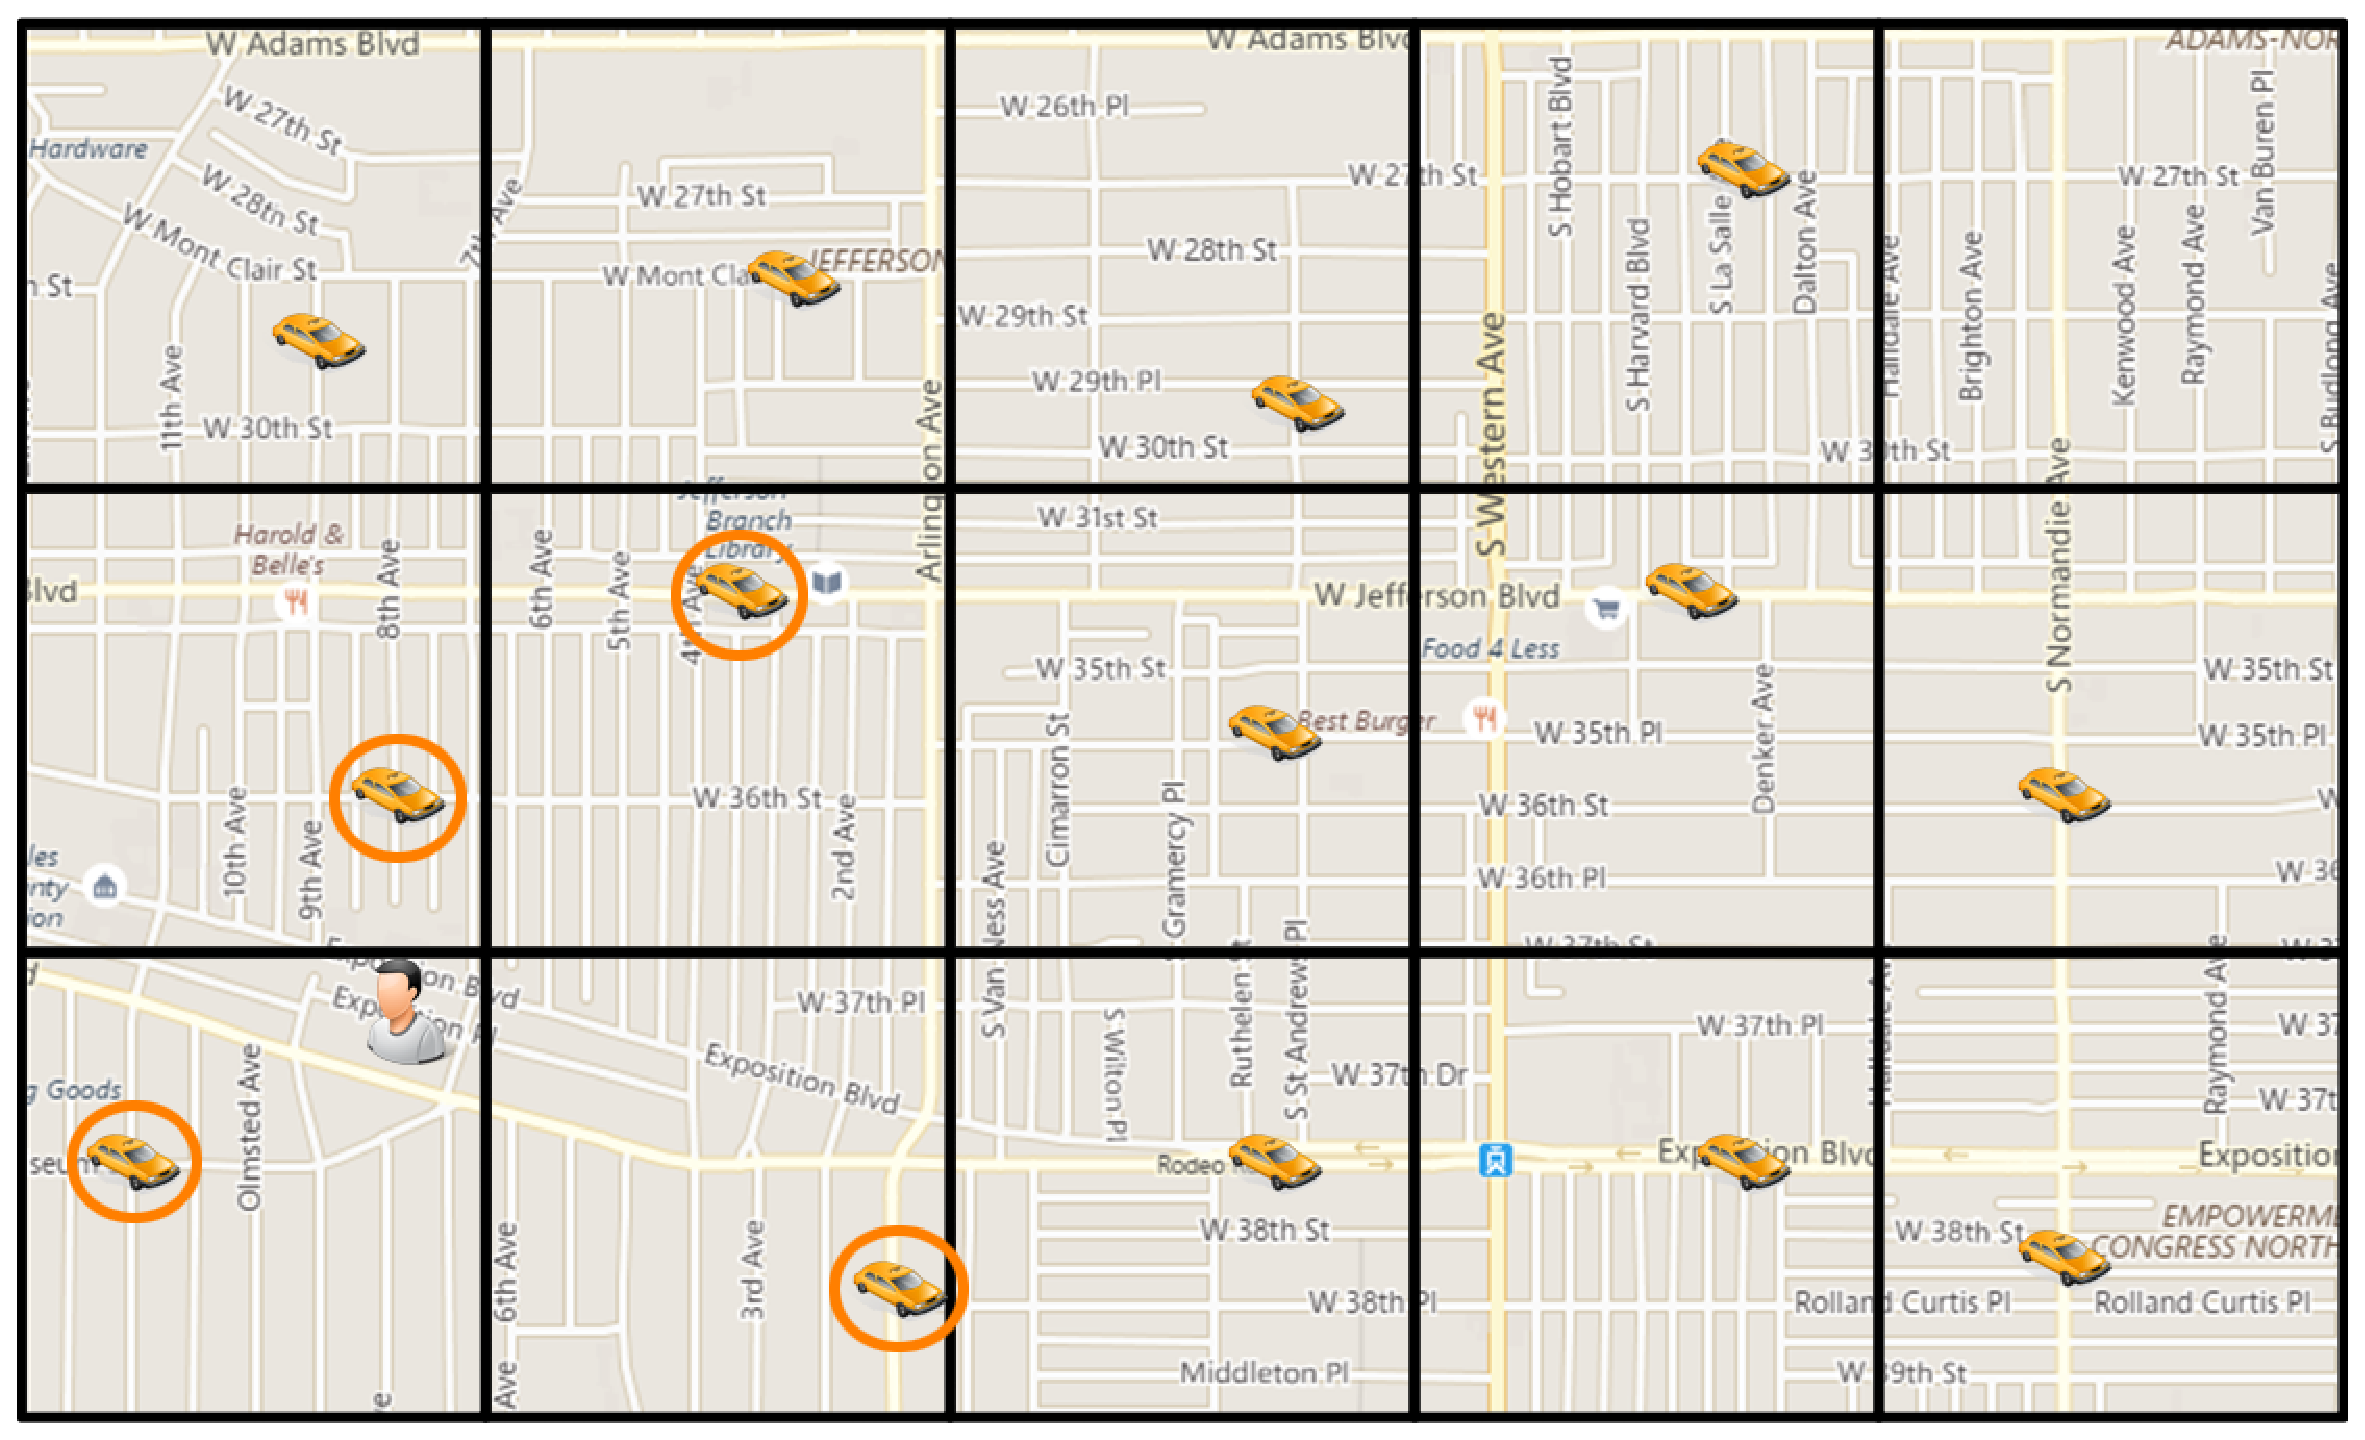
\includegraphics[width = 0.95\columnwidth]{dispatch5.eps}
\end{figure}
}
\end{frame}

\begin{frame}\frametitle{Bid Computation}
\begin{columns}

\column{0.7\textwidth}
\vspace{-0.3in}
\only<1>{
\vspace{-0.15in}
\begin{figure}
	\centering
    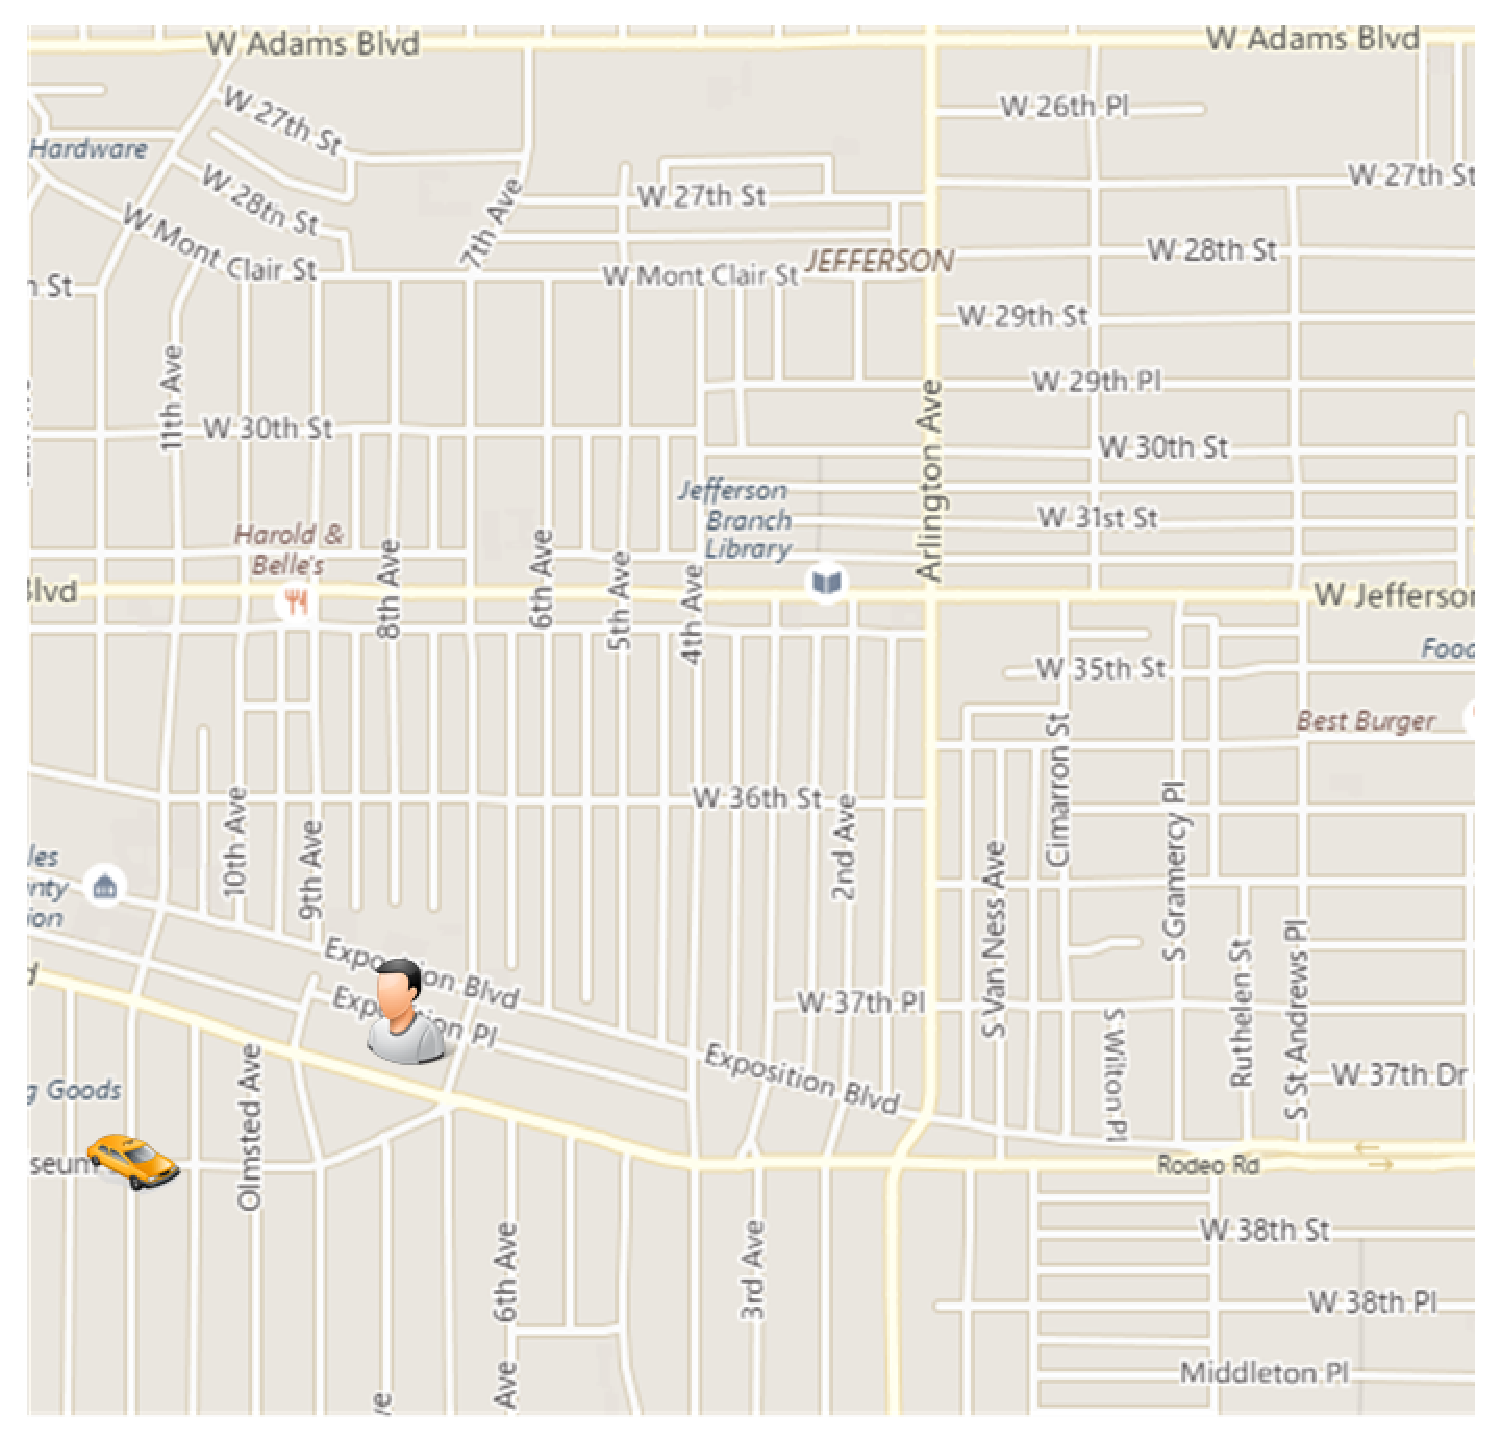
\includegraphics[width = 0.95\columnwidth]{bid1.eps}
\end{figure}
}
\only<2>{
\vspace{-0.15in}
\begin{figure}
	\centering
    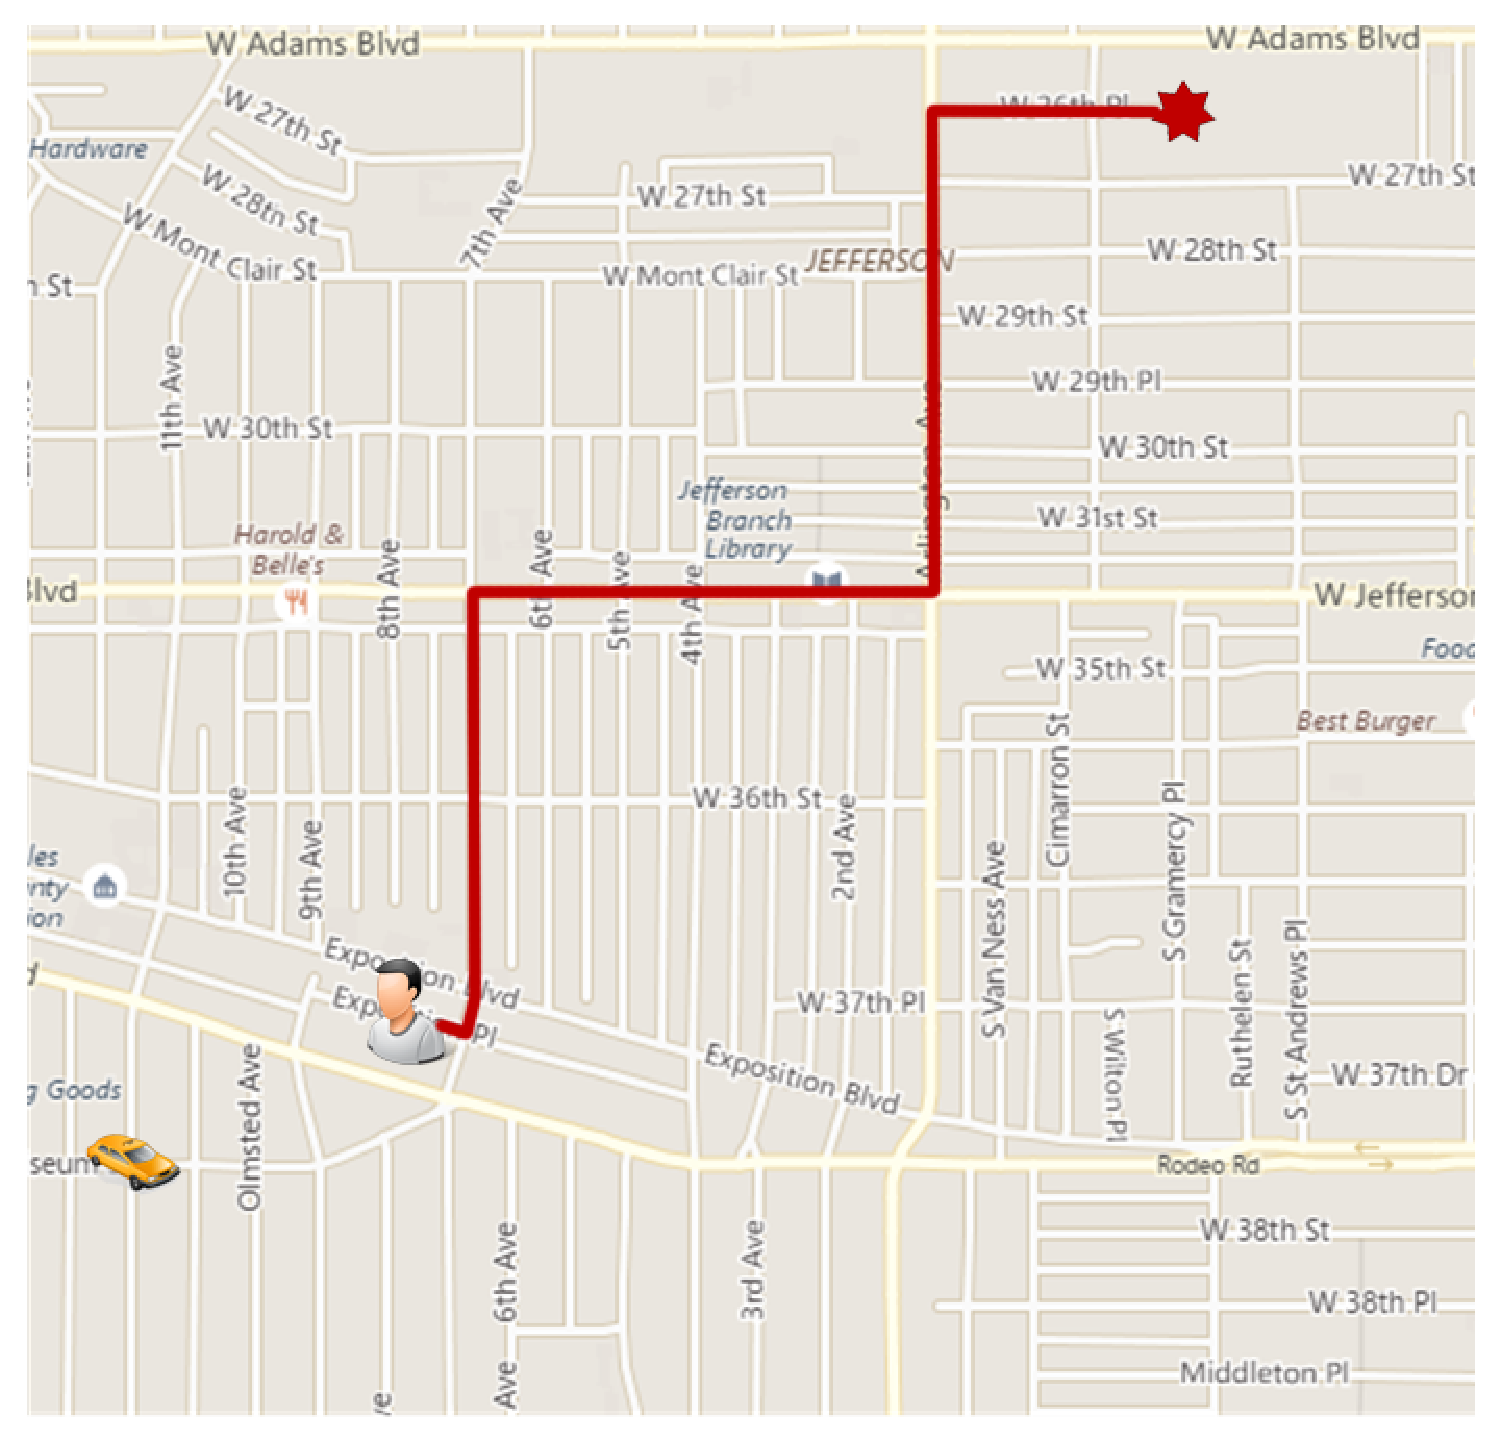
\includegraphics[width = 0.95\columnwidth]{bid2.eps}
\end{figure}
}
\only<3>{
\vspace{-0.15in}
\begin{figure}
	\centering
    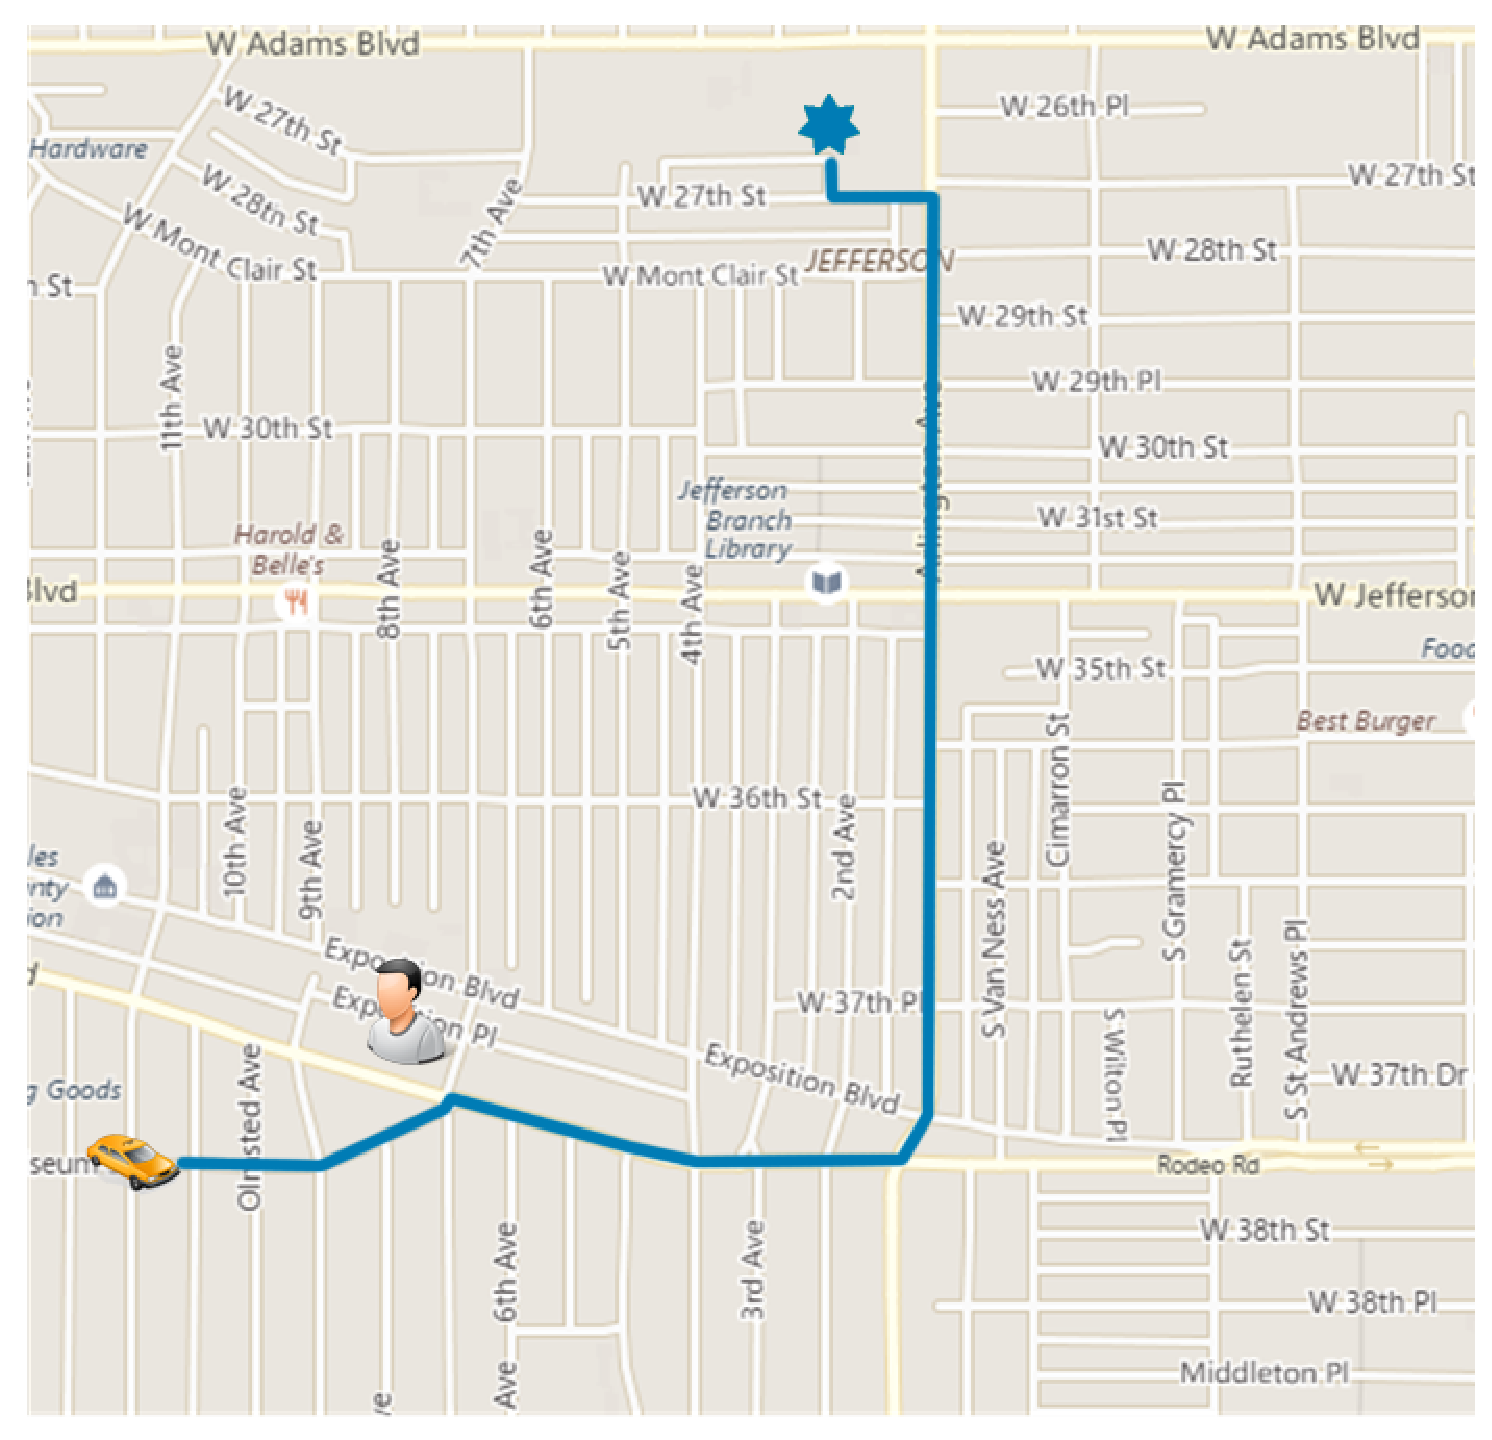
\includegraphics[width = 0.95\columnwidth]{bid3.eps}
\end{figure}
}
\only<4->{
\vspace{-0.15in}
\begin{figure}
	\centering
    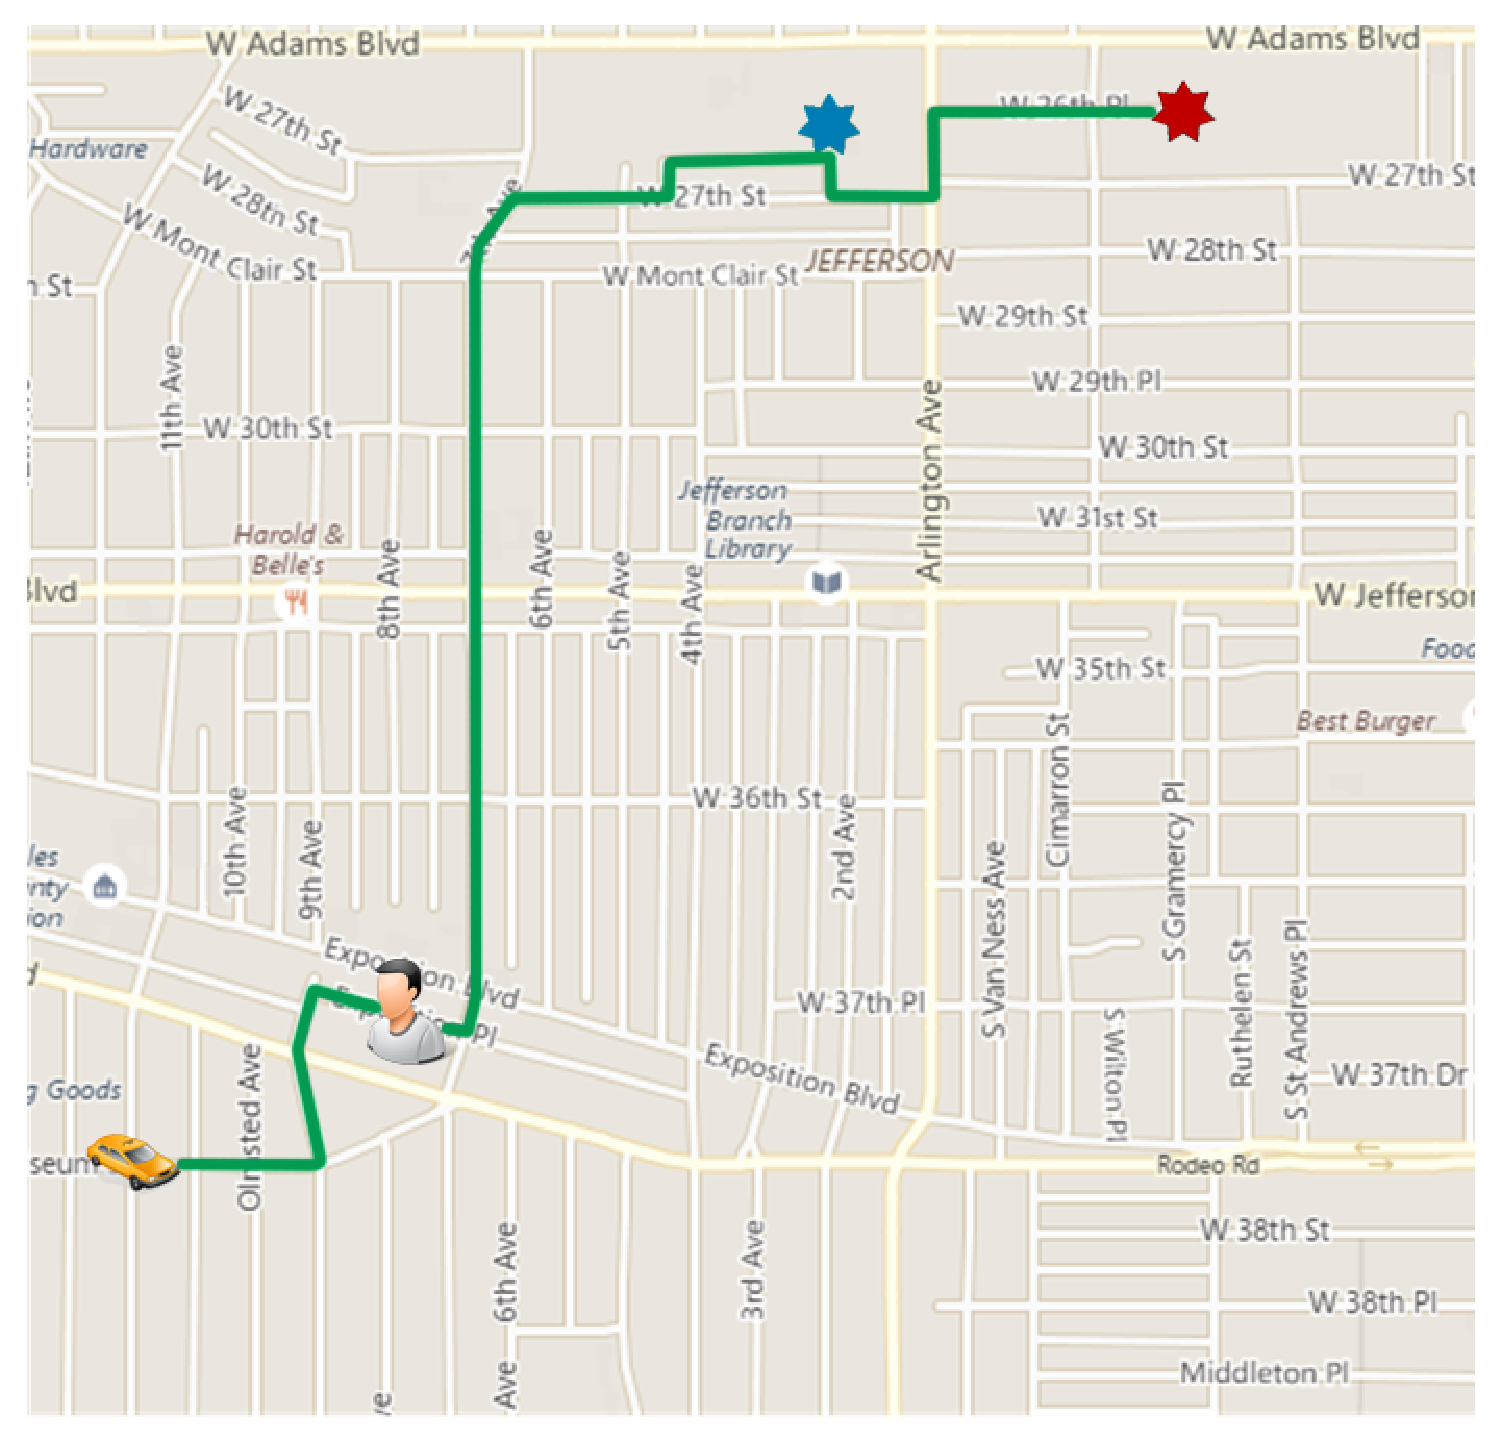
\includegraphics[width = 0.95\columnwidth]{bid4.eps}
\end{figure}
}
\column{0.3\textwidth}
\only<2->{using \textcolor{red}{PATH} we get the \textit{base fare} for the new request\\}
\vspace{0.15in}
\only<3->{using \textcolor{blue}{PATH} we get the \textit{current profit}\\}
\vspace{0.15in}
\only<4->{\textit{diff(\textcolor{green}{route}, \textcolor{red}{route})} gives $\Delta d$ for new request\\}
\vspace{0.15in}
\only<5->{
\begin{alertblock}{Bid}
new profit - \\ current profit
\end{alertblock}
}
\end{columns}
\end{frame}

\section{Experiments}
\frame{\frametitle{Outline}\tableofcontents[currentsection]}

\begin{frame}\frametitle{Setup}
\begin{itemize}
\item Data Set: New York City's Taxi data set
\only<1>{
\begin{itemize}
\item<1> 40K drivers \& 500K trips per day
\item<1> pickup/dropoff points, request time
\end{itemize}
}
\item<2-> Algorithms:
\only<2>{
\begin{itemize}
\item<2> APART
\item<2> TREE (shortest traveled distance) [1]
\item<2> NN (closest driver)
\end{itemize}
}
\item<3-> Parameters:
\only<3>{
\vspace{-0.25in}
\begin{table}
	\begin{center}
		\begin{tabular}{|c|c|}
			\hline
			Parameter & Values \\
			\hline \hline
			Max Wait Time (w) & 3min, \textbf{6min}, 9min, 12min, 15min, 20min \\ 
			\hline
			\# of Drivers & 1000, 2000, \textbf{5000},  10000, 20000\\ 
			\hline
			Max Passengers (n) & 2, 3, \textbf{4}, 5, 6 \\
			\hline
			Max Allowed Detour ($\epsilon$) & 25\%, \textbf{50\%}, 75\%, 100\%\\
			\hline
		\end{tabular}
	\end{center}
\end{table}
}
\item<4-> Pricing Model:
\only<4>{
\begin{equation*}
	\begin{split}
		F(d) & = 2 \times d \\
		\forall r, f_r(\Delta d_r) & = 1 - (0.25 \times \Delta d_r^2) \\
		\forall v, g_v(d)  & = 1.5 \times d
	\end{split}
\end{equation*}
}
\end{itemize}
\only<2>{
\vspace{1in}
\tiny{[1] Y. Huang, F. Bastani, R. Jin, and X. S. Wang, “Large scale real-time ridesharing with service guarantee on road networks,” Proceedings of the VLDB Endowment, vol. 7, no. 14, pp. 2017–2028, 2014.}
}
\end{frame}

\begin{frame}\frametitle{Algorithm Comparison}
\begin{columns}
\column{0.5\textwidth}
\vspace{-0.4in}
\begin{figure}
	\centering
    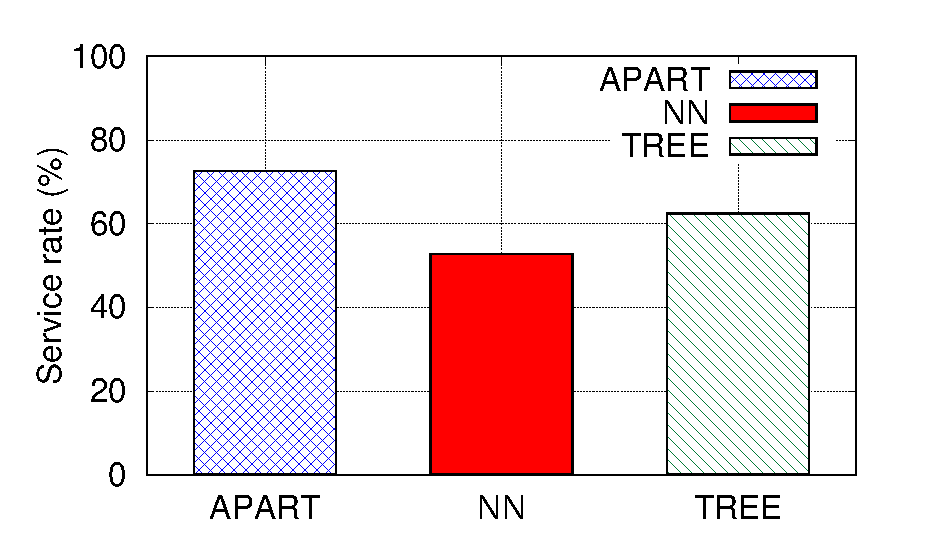
\includegraphics[width = 0.95\columnwidth]{default_sr.eps}
    \vspace{-0.08in}
    \small{\textit{\textbf{Service Rate}}}
\end{figure}
\column{0.5\textwidth}
\vspace{-0.4in}
\begin{figure}
	\centering
    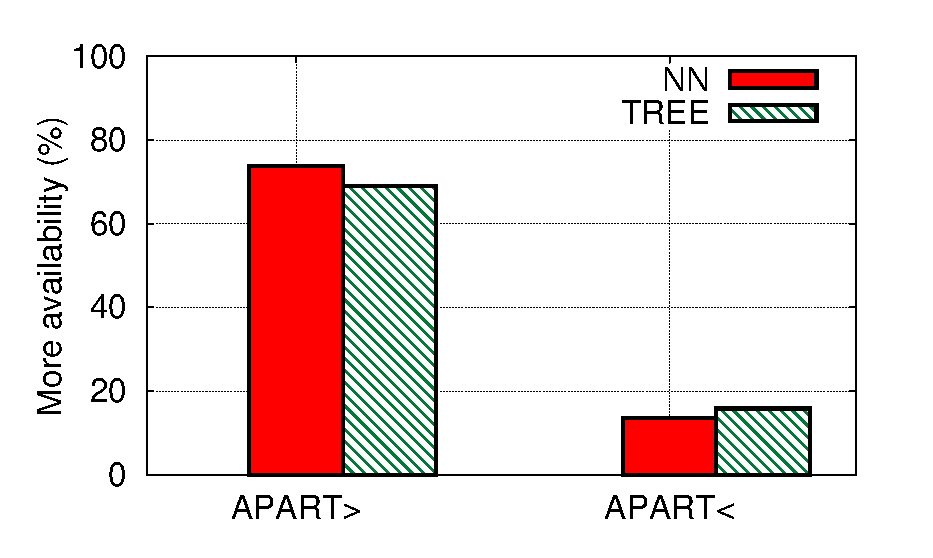
\includegraphics[width = 0.95\columnwidth]{availability.eps}
    \vspace{-0.08in}
    \small{\textit{\textbf{Driver Availability}}}
\end{figure}
\end{columns}
\begin{columns}
\column{0.5\textwidth}
\vspace{-0.1in}
\begin{figure}
	\centering
    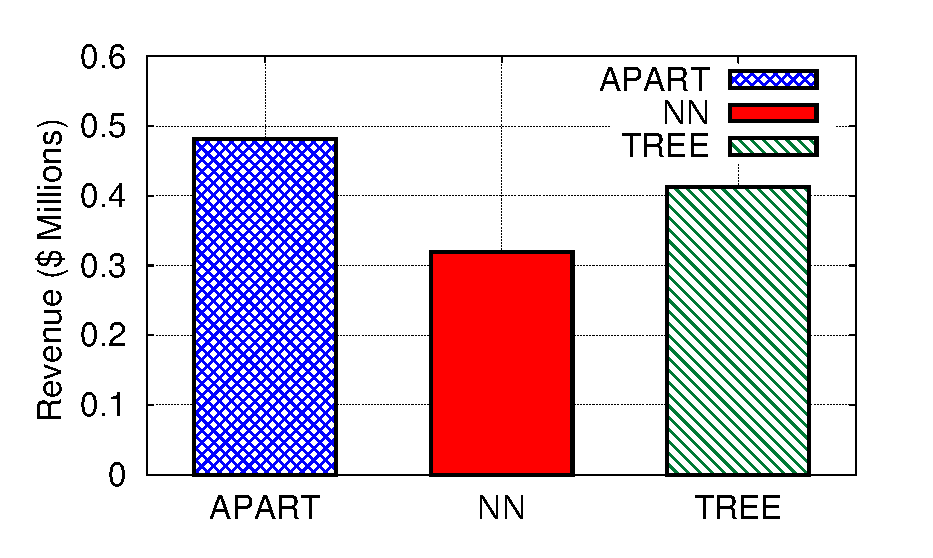
\includegraphics[width = 0.95\columnwidth]{default_rev.eps}
    \vspace{-0.08in}
    \small{\textit{\textbf{Revenue}}}
\end{figure}
\column{0.5\textwidth}
\vspace{-0.1in}
\begin{figure}
	\centering
    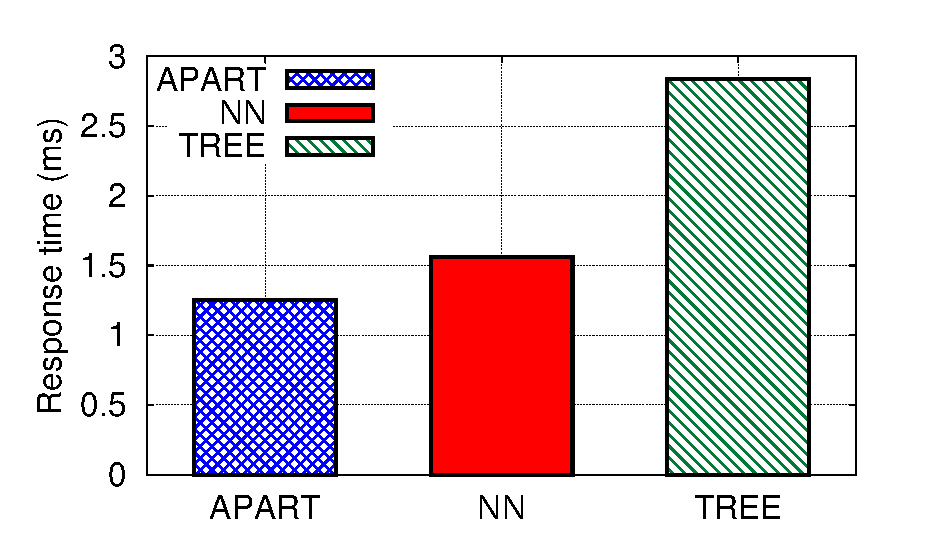
\includegraphics[width = 0.95\columnwidth]{default_rp.eps}
    \vspace{-0.08in}
    \small{\textit{\textbf{Response Time}}}
\end{figure}
\end{columns}
\end{frame}

\begin{frame}\frametitle{Pricing Model Comparison}
If we use the frame work in [2]:
\begin{equation*}
c.d_1 + (1+\alpha).c.d_2
\end{equation*}
\vspace{-0.3in}
\begin{columns}
\column{0.5\textwidth}
\begin{figure}
	\centering
    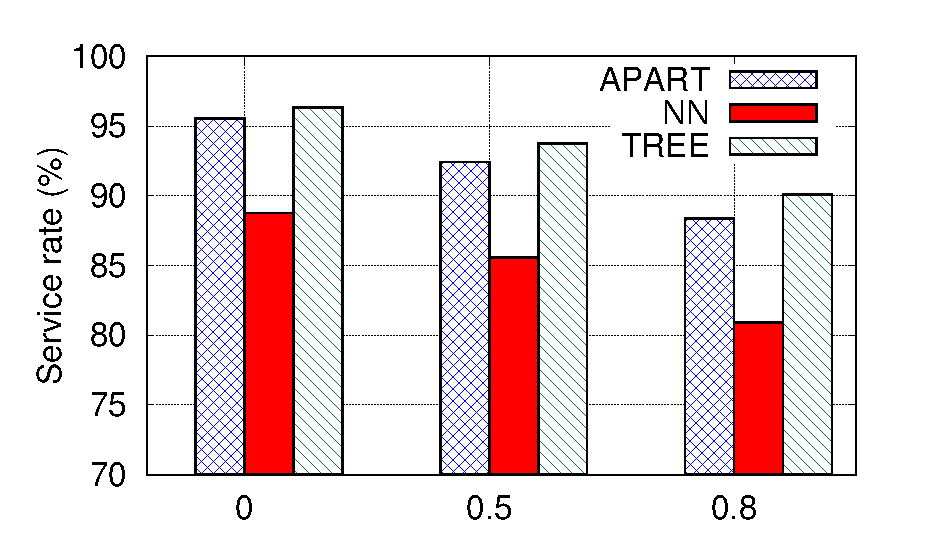
\includegraphics[width = 0.95\columnwidth]{saved.eps}
    \vspace{-0.1in}
    \small{$\alpha$}\\
    \small{\textbf{\textit{Users that Saved Money}}}
\end{figure}
\column{0.5\textwidth}
\begin{figure}
	\centering
    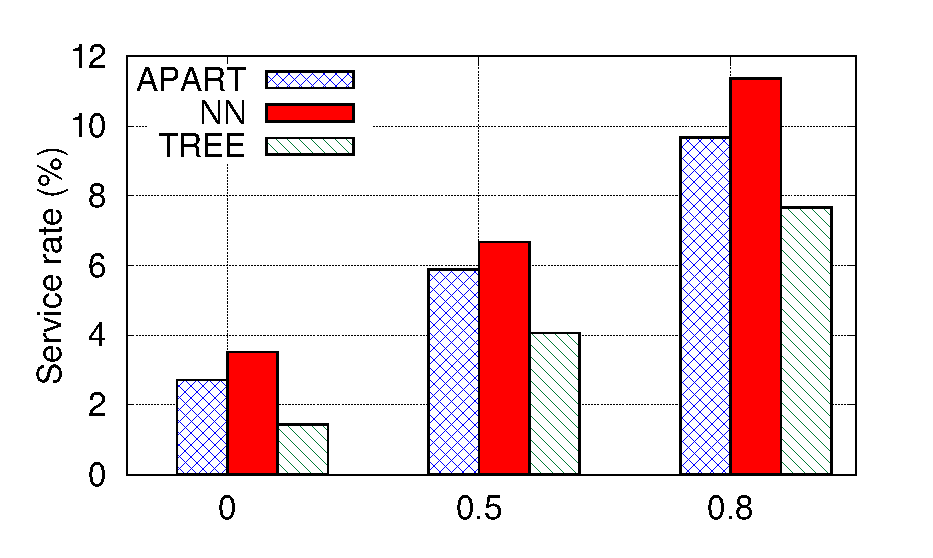
\includegraphics[width = 0.95\columnwidth]{lost.eps}
    \vspace{-0.1in}
    \small{$\alpha$}\\
    \small{\textbf{\textit{Users that Lost Money}}}
\end{figure}
\end{columns}
\vspace{0.4in}
\tiny{[2] S. Ma, Y. Zheng, and O. Wolfson, “T-share: A large-scale dynamic taxi ridesharing service,” in Data Engineering (ICDE), 2013 IEEE 29th International Conference on}
\end{frame}

\begin{frame}\frametitle{Effect of Profiles}
\begin{itemize}
\item $APART_T$: $f_T(\Delta d_r) = \frac{1}{(\Delta d_r + 1)}$
\item $APART_R$: $f_R(\Delta d_r) = 1 -  (\frac{\Delta d_r}{max \delta})$ 
\end{itemize}
\only<1>{
\begin{columns}
  \column{.5\textwidth}
  \begin{center}
    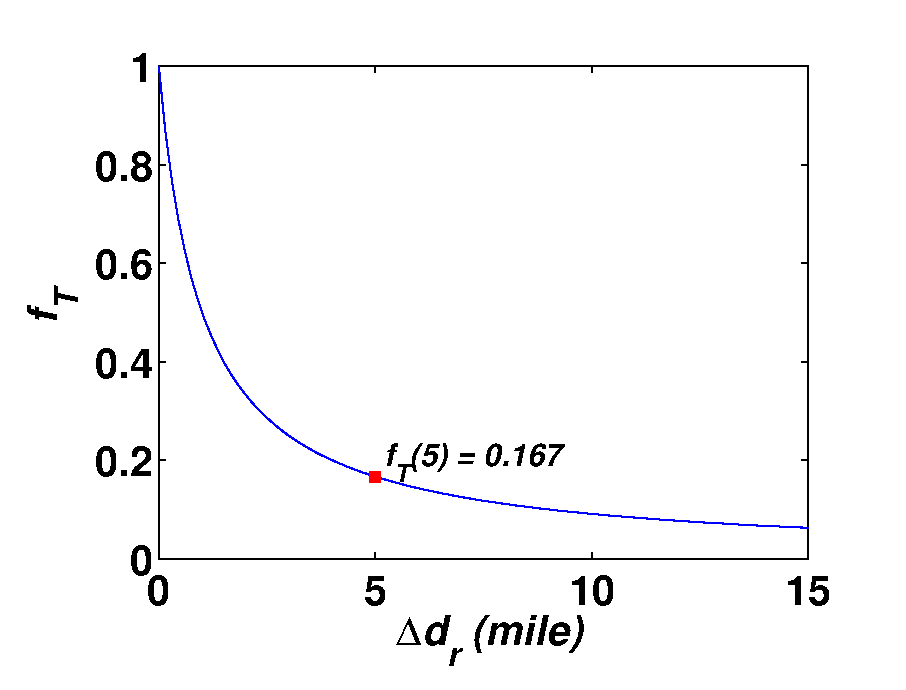
\includegraphics[width=0.8\columnwidth]{f_T.eps}
  \end{center}
  \column{.5\textwidth}
  \begin{center}
    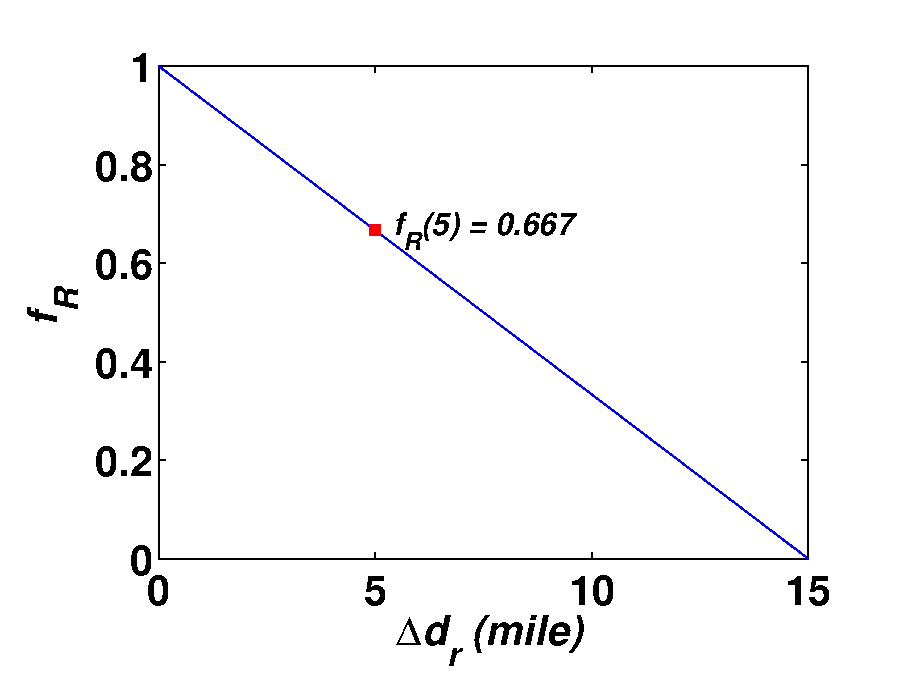
\includegraphics[width=0.8\columnwidth]{f_R.eps}   
  \end{center}
\end{columns} 
}
\only<2->{
\begin{figure}
	\centering
    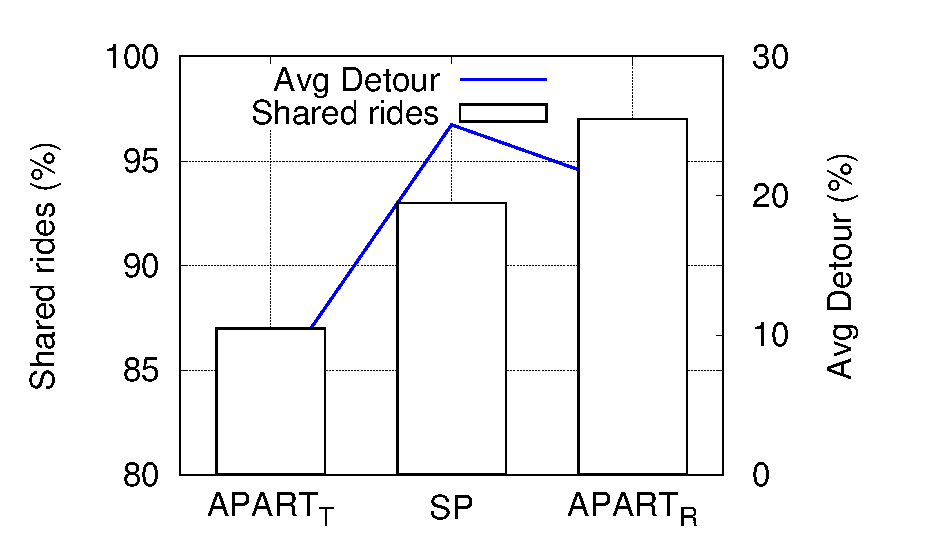
\includegraphics[width = 0.55\columnwidth]{quality.eps}\\
    \vspace{-0.075in}
    \small{\textit{\textbf{Effect of Profiles}}}
\end{figure}
}
\end{frame}

\section*{Q \& A}
\begin{frame}\frametitle{Questions}
\begin{center}
	
\includegraphics[scale=0.3]{QandA.jpg}
\end{center}
\end{frame}




\end{document}